\documentclass[aspectratio=169,xcolor=svgnames]{beamer}
%\documentclass{beamer}
%%%CHOOSE ASPECT RATIO ABOVE%%%

% \usetheme{LU-spfaff}

%\usepackage[utf8]{inputenc}
\usepackage[british]{babel}
\usepackage{grffile}
\usepackage{minted}
\usepackage{csquotes}
\usepackage{tikz}
\usepackage{libertine}
\usepackage{fancyvrb}
\usepackage{xspace}

\usepackage{emoji}

% \usefonttheme{serif}

\usetikzlibrary{tikzmark}
\usetikzlibrary{arrows.meta}
\usetikzlibrary{positioning}
\usetikzlibrary{decorations.pathmorphing, decorations.pathreplacing, decorations.shapes,}

\tikzstyle{every picture} += [remember picture]

\setminted[java]{autogobble=true,bgcolor=LightGray,linenos}
\setminted[python]{autogobble=true,bgcolor=LightGray,linenos}

\setmonofont{Fira Code}
\usepackage[sfdefault]{FiraSans}
\usepackage{fontspec}
\newfontfamily{\NotoEmoji} {Noto Color Emoji}[Renderer=Harfbuzz]
\newfontfamily{\DejaSans} {DejaVu Sans}
\newfontfamily{\NotoSans} {Noto Sans}

\title[]{Bayesian Statistics}

% \titlecolor{LUGreen} % Choose between LUPink, LULBlue, LUIvory, LUGreen
%\titleimage{\includegraphics[scale=.5]{astro.png}}
% \titleimage{\includegraphics[scale=.6]{lumainb.jpg}}
\author{Noric Couderc}
% \subtitle{Subtitles are currently limited to one line}
\date{\today}
\institute{Lund University\\Department of Computer Science}

\AtBeginSection[]{
  \begin{frame}
  \vfill
  \centering
  \begin{beamercolorbox}[sep=8pt,center,shadow=true,rounded=true]{title}
    \usebeamerfont{title}\textbf{\insertsectionhead}\par%
  \end{beamercolorbox}
  \vfill
  \end{frame}
}

\setbeamertemplate{footline}[frame number]

\begin{document}

\maketitle

\begin{frame}{About Me}
  \begin{columns}
    \column{0.5\textwidth}
    My name is Noric

    \begin{itemize}
    \item 5th year PhD student
    \item From: Digne les Bains, France
    \item Topics: Dynamic program analysis, performance engineering
    \item Supervisors: Christoph Reichenbach, Emma Söderberg
    \end{itemize}

    \column{0.5\textwidth}
    \includegraphics[width=\columnwidth]{/home/noric/Pictures/moi.jpg}

  \end{columns}
\end{frame}

\begin{frame}
  \begin{block}{My job}
  \begin{enumerate}
  \item <2->Run programs
  \item <3->Count stuff \emoji{stopwatch}
  \end{enumerate}
  \end{block}
\end{frame}

\section{Performance Example}

\begin{frame}
  \begin{figure}[ht]
    \centering
    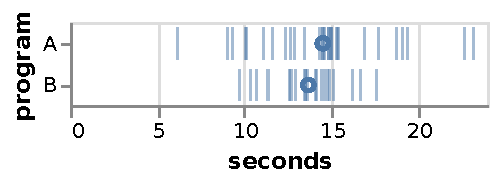
\includegraphics[width=\textwidth]{figures/samples_a_b.pdf}
    \caption{Which program is faster?}
  \end{figure}
\end{frame}

\begin{frame}
  \center
  Can we trust the means we compute?
\end{frame}

\begin{frame}
  \center
  \emoji{test-tube} Simulate and test \emoji{test-tube}
\end{frame}

\begin{frame}{Normal Distribution}
  \begin{figure}[ht]
    \centering
    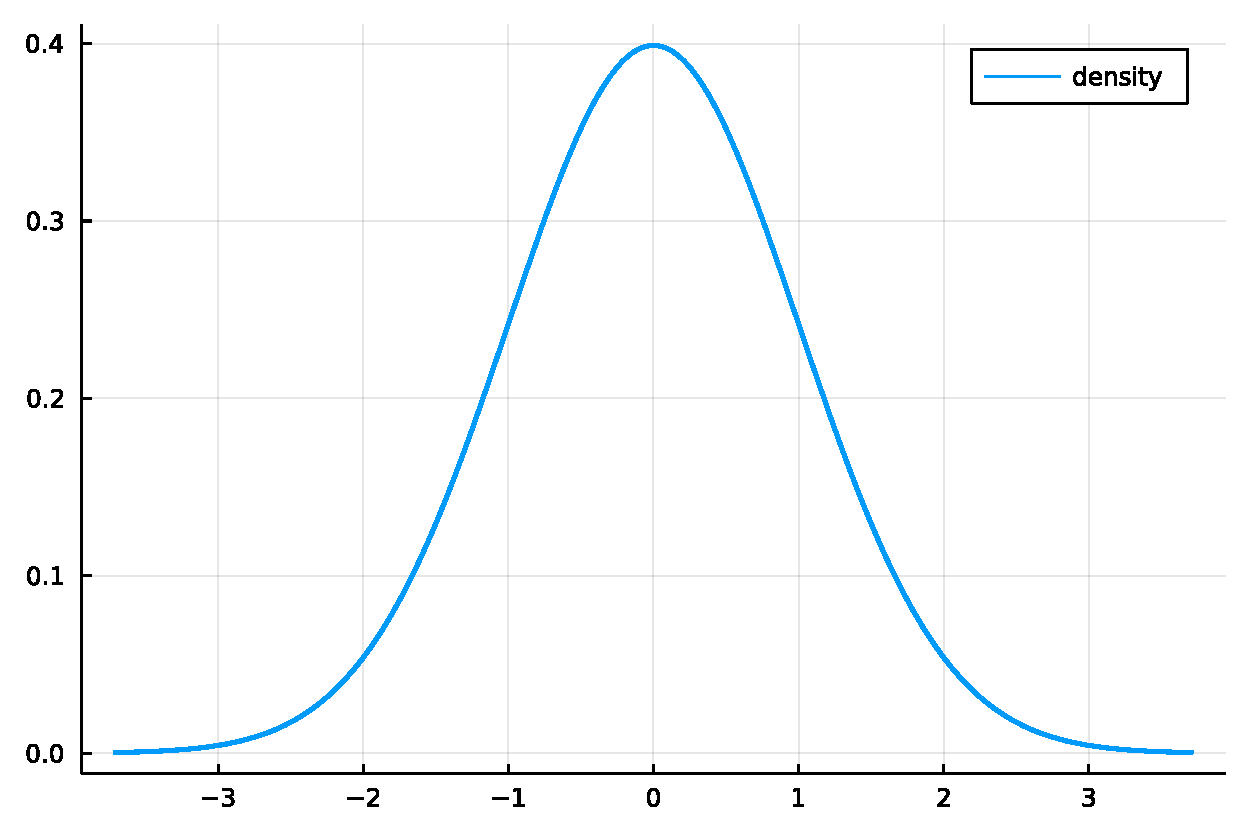
\includegraphics[width=0.8\textwidth]{figures/normal_distribution.pdf}
    % \caption{\label{fig:label} }
  \end{figure}
\end{frame}

\begin{frame}{Sampling}
  % Show ``the mean'' doesn't really exist, it has some error!
  \begin{figure}[ht]
    \centering
    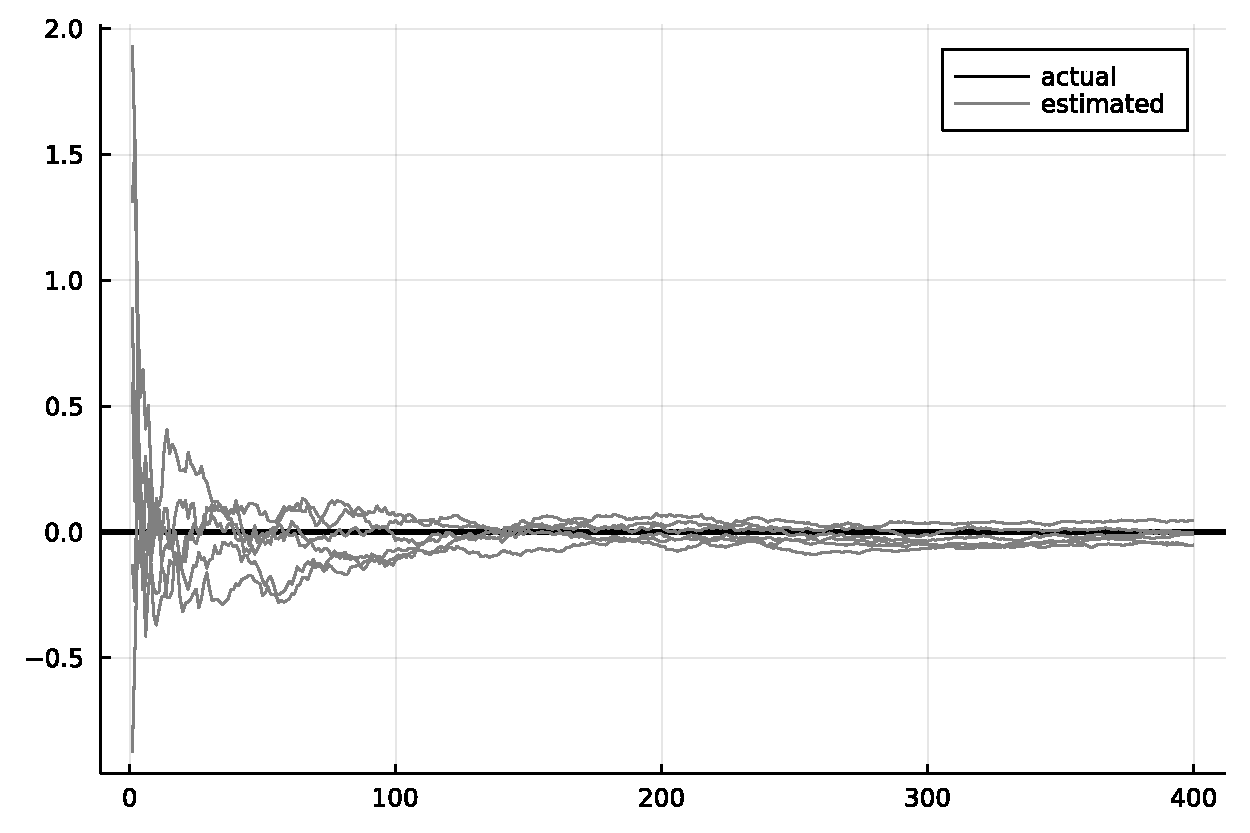
\includegraphics[width=0.8\textwidth]{figures/mean_error.pdf}
  \end{figure}
\end{frame}

\begin{frame}{Sampling}
  \begin{columns}
    \begin{column}{0.4\textwidth}
    \begin{figure}[ht]
        \centering
        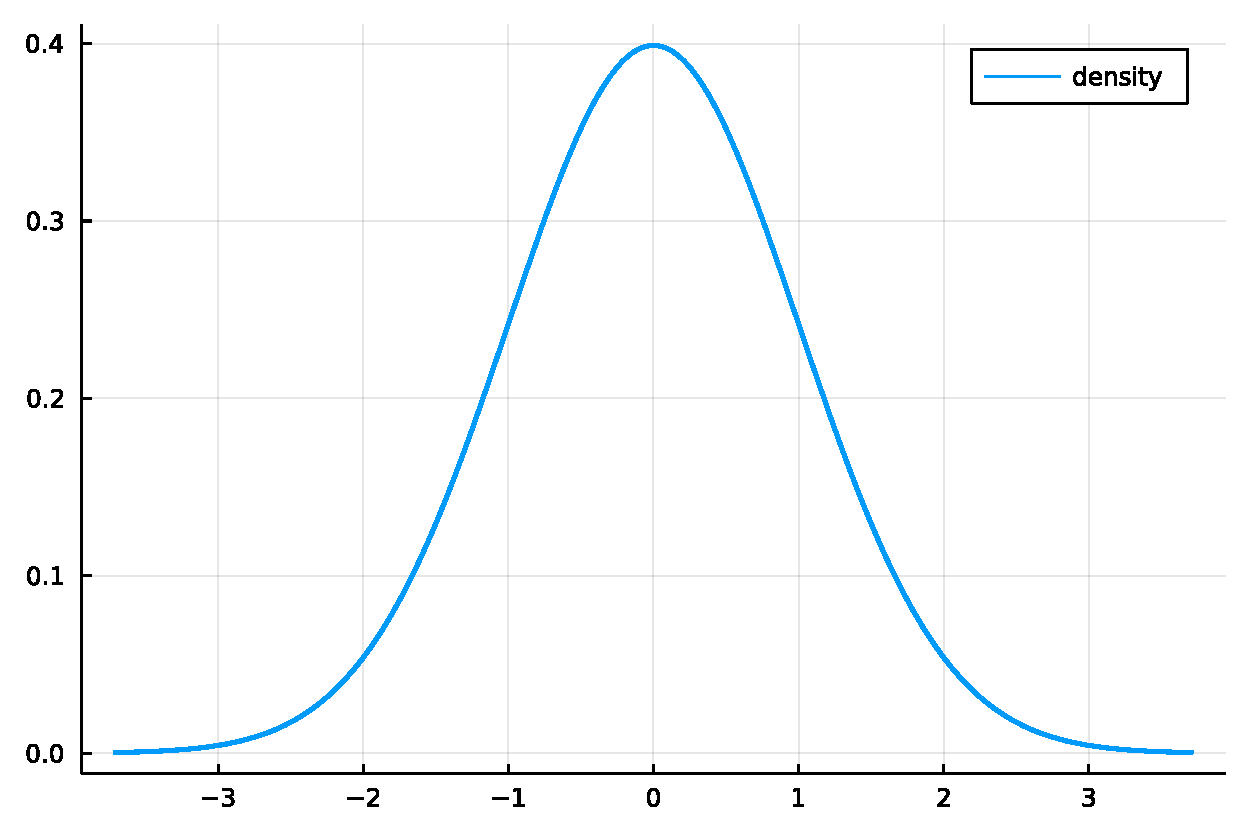
\includegraphics[width=\textwidth]{figures/normal_distribution.pdf}
        % \caption{\label{fig:label} }
    \end{figure}
    \end{column}
    \begin{column}{0.6\textwidth}
      \begin{figure}[ht]
        \centering
        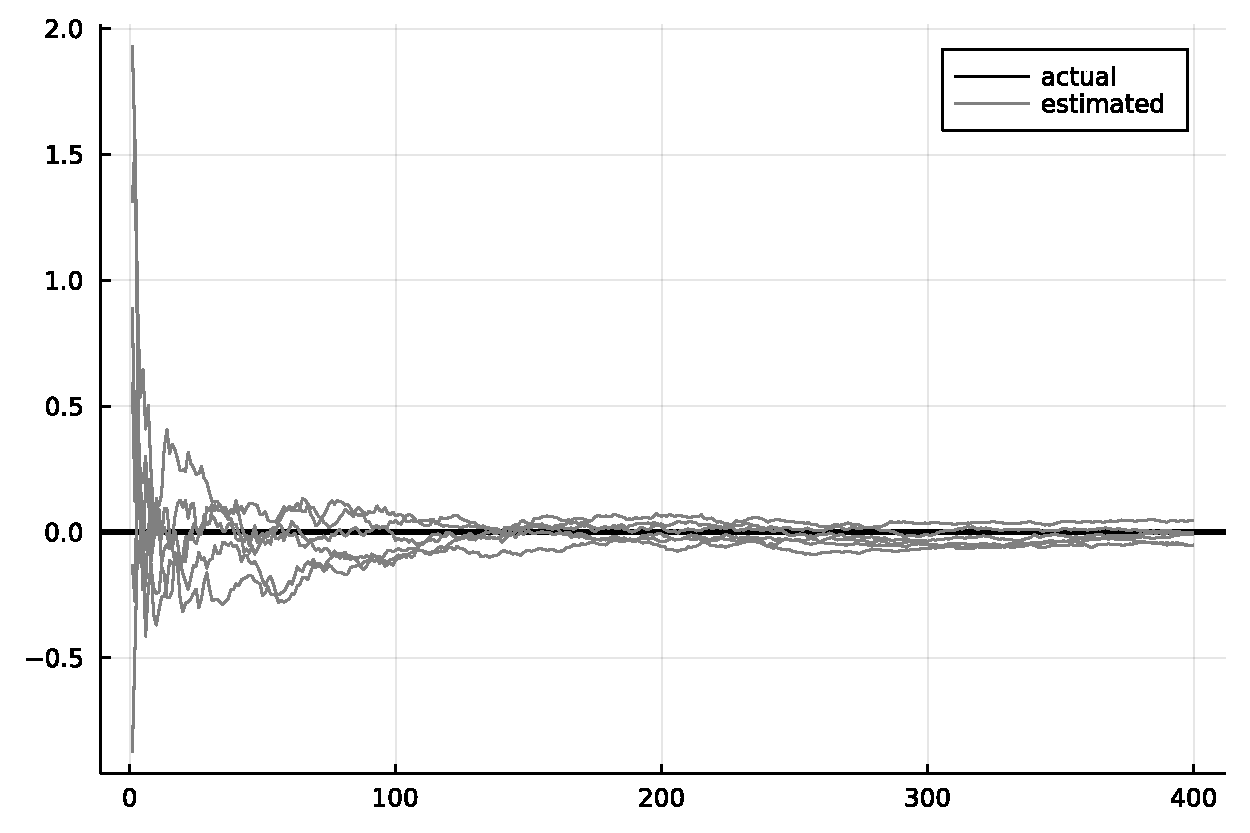
\includegraphics[width=\textwidth]{figures/mean_error.pdf}
      \end{figure}
    \end{column}
  \end{columns}
\end{frame}

\begin{frame}
  \huge
  \center
  Statistics

  Working with numbers you \textbf{can't trust}
\end{frame}

\begin{frame}
  \begin{figure}[ht]
    \centering
    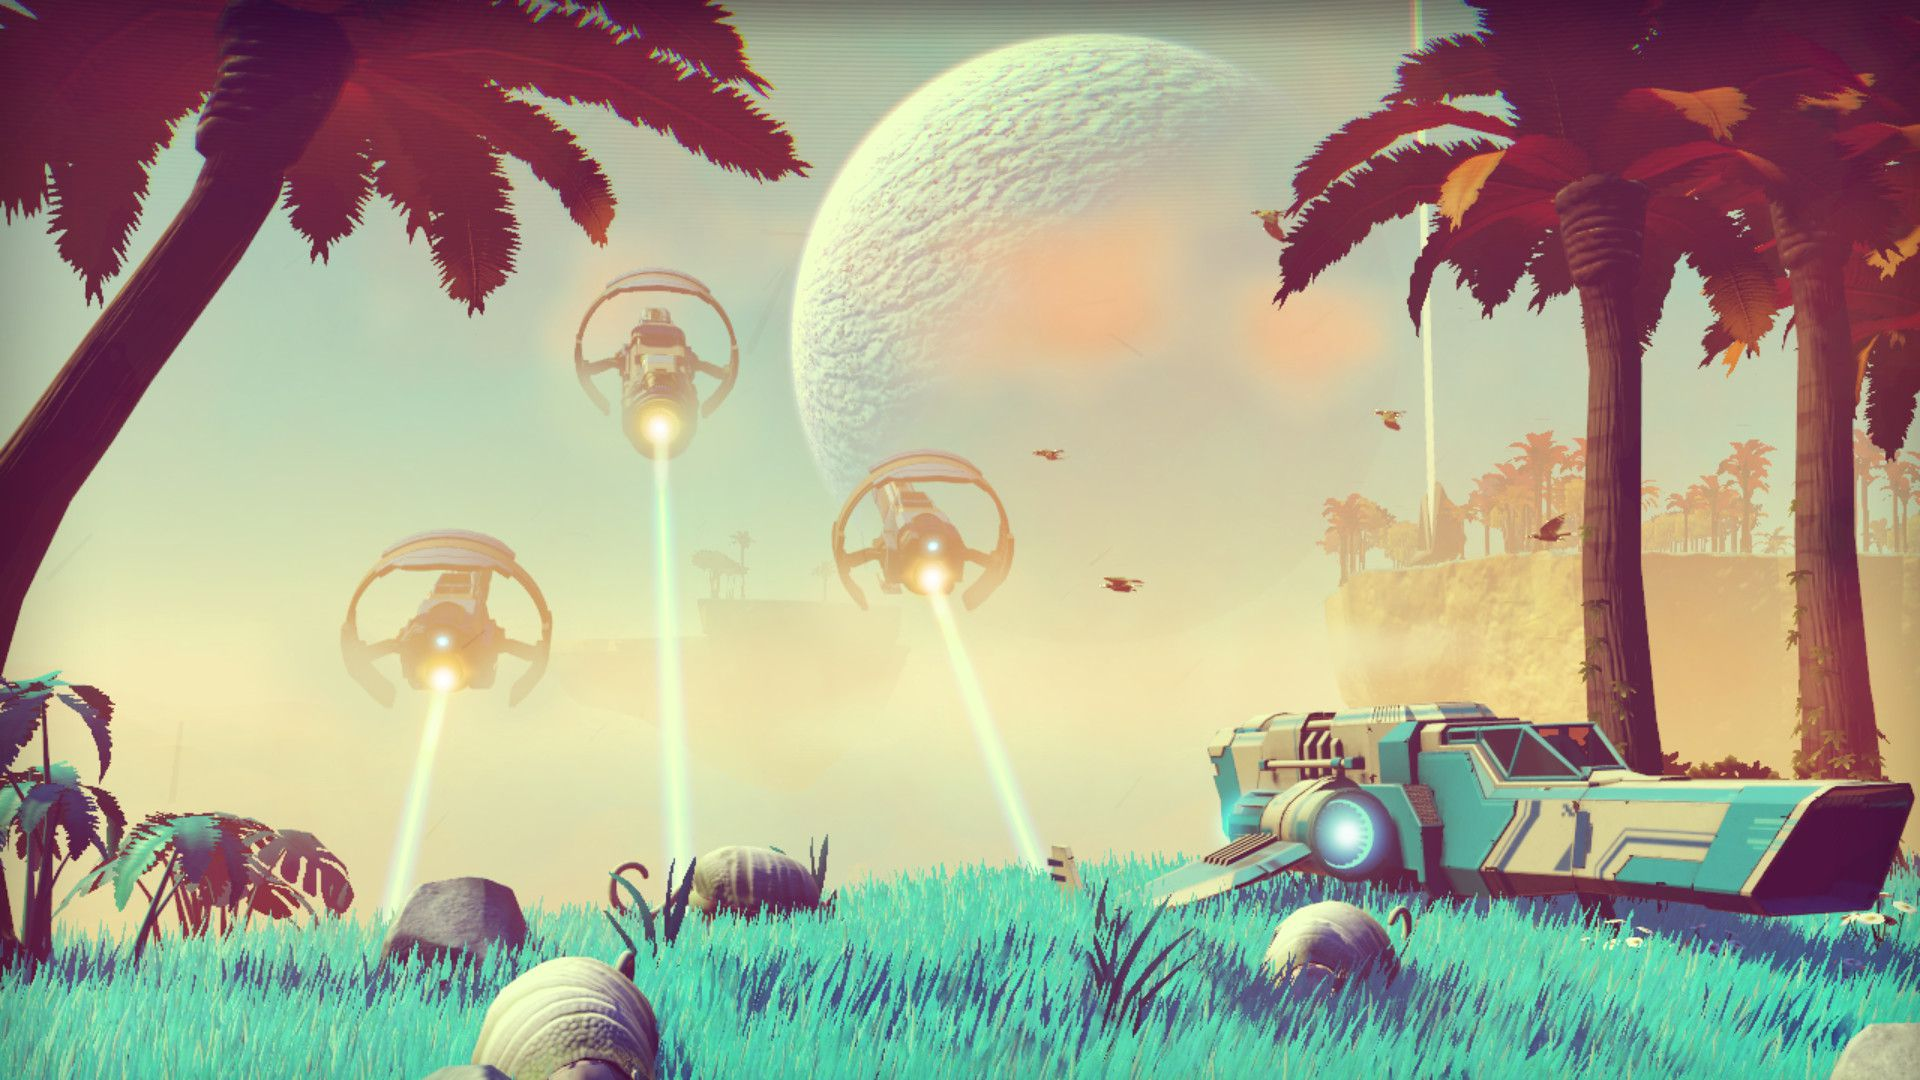
\includegraphics[width=0.8\textwidth]{figures/no-mans-sky-screenshot.jpg}
    \caption{No Man's Sky by Hello Games}
  \end{figure}
\end{frame}

\begin{frame}
  \begin{columns}
    \begin{column}{0.5\textwidth}
      \center
      \begin{tikzpicture}[>=Stealth]
        \draw[thick] (0, 2) -- (0, -2);
        \fill (-2, 0) circle[radius=2pt] node[above] {fixed};

        \draw (-2, 0) -- (0, 0);

        \draw (0,0) -- (2,0) circle[radius=2pt] ;
        \draw (0,0) -- (2,0.5) circle[radius=2pt] ;
        \draw (0,0) -- (2,-0.4) circle[radius=2pt] ;
        \draw (0,0) -- (2,1.2) circle[radius=2pt] ;
        \draw (0,0) -- (2,-1.3) circle[radius=2pt] ;

        \draw[decorate, decoration={coil, aspect=0}] (1.75, 2) -- (1.75,-2);
        \draw[decorate, decoration={coil, aspect=0}] (2.25, 2) -- (2.25,-2);

        \draw[->,thick] (-2, -3) -- node[midway,above] {Simulation} (2, -3);
      \end{tikzpicture}
    \end{column}
    \begin{column}{0.5\textwidth}
      \center
      \begin{tikzpicture}[>=Stealth]
        \draw[thick] (0, 2) -- (0, -2);
        \draw(-2, 0) circle[radius=2pt];
        \draw(-2, 0.1) circle[radius=2pt];
        \draw(-2, 0.07) circle[radius=2pt];
        \draw(-2, -0.03) circle[radius=2pt];
        \draw(-2, -0.12) circle[radius=2pt];

        \draw (-2, 0) -- (0, 0);

        \draw[decorate, decoration={coil, aspect=0}] (-1.75, 2) -- (-1.75,-2);
        \draw[decorate, decoration={coil, aspect=0}] (-2.25, 2) -- (-2.25,-2);

        \draw[fill=black] (2,0) circle[radius=2pt] -- (0,0);
        \draw[fill=black] (2,0.5) circle[radius=2pt] -- (0,0);
        \draw[fill=black] (2,-0.4) circle[radius=2pt] -- (0,0);
        \draw[fill=black] (2,1.2) circle[radius=2pt] -- (0,0);
        \draw[fill=black] (2,-1.3) circle[radius=2pt] node[below] {fixed} -- (0,0);


        \draw[->,thick] (2, -3) -- node[midway,above] {Inference} (-2, -3);
      \end{tikzpicture}
    \end{column}
  \end{columns}
\end{frame}

\begin{frame}
  \begin{itemize}
  \item \textbf{Prediction:} You know the inputs and the function, but not the outputs
  \item \textbf{Inference:} You know the outputs and the function, but not the inputs
  \item \textbf{Learning:} You know the inputs and the outputs, but not the function
  \end{itemize}
\end{frame}

\begin{frame}
  \center
  \huge
  Bayesian inference

  \small
  Make fuzzy estimates of things
\end{frame}

\section{The Crush Problem}

\newcommand{\love}[0]{{\NotoEmoji ❤️}\xspace}
\newcommand{\flowers}[0]{{\emoji{bouquet}}\xspace}

\begin{frame}{The Crush Problem}
  \begin{columns}
    \begin{column}{0.4\textwidth}
      \begin{itemize}
      \item You observed \flowers.
      \item What is $P(\text{\love}|\text{\flowers})$?
      \end{itemize}
    \end{column}
    \begin{column}{0.6\textwidth}
      \begin{figure}[ht]
        \centering
        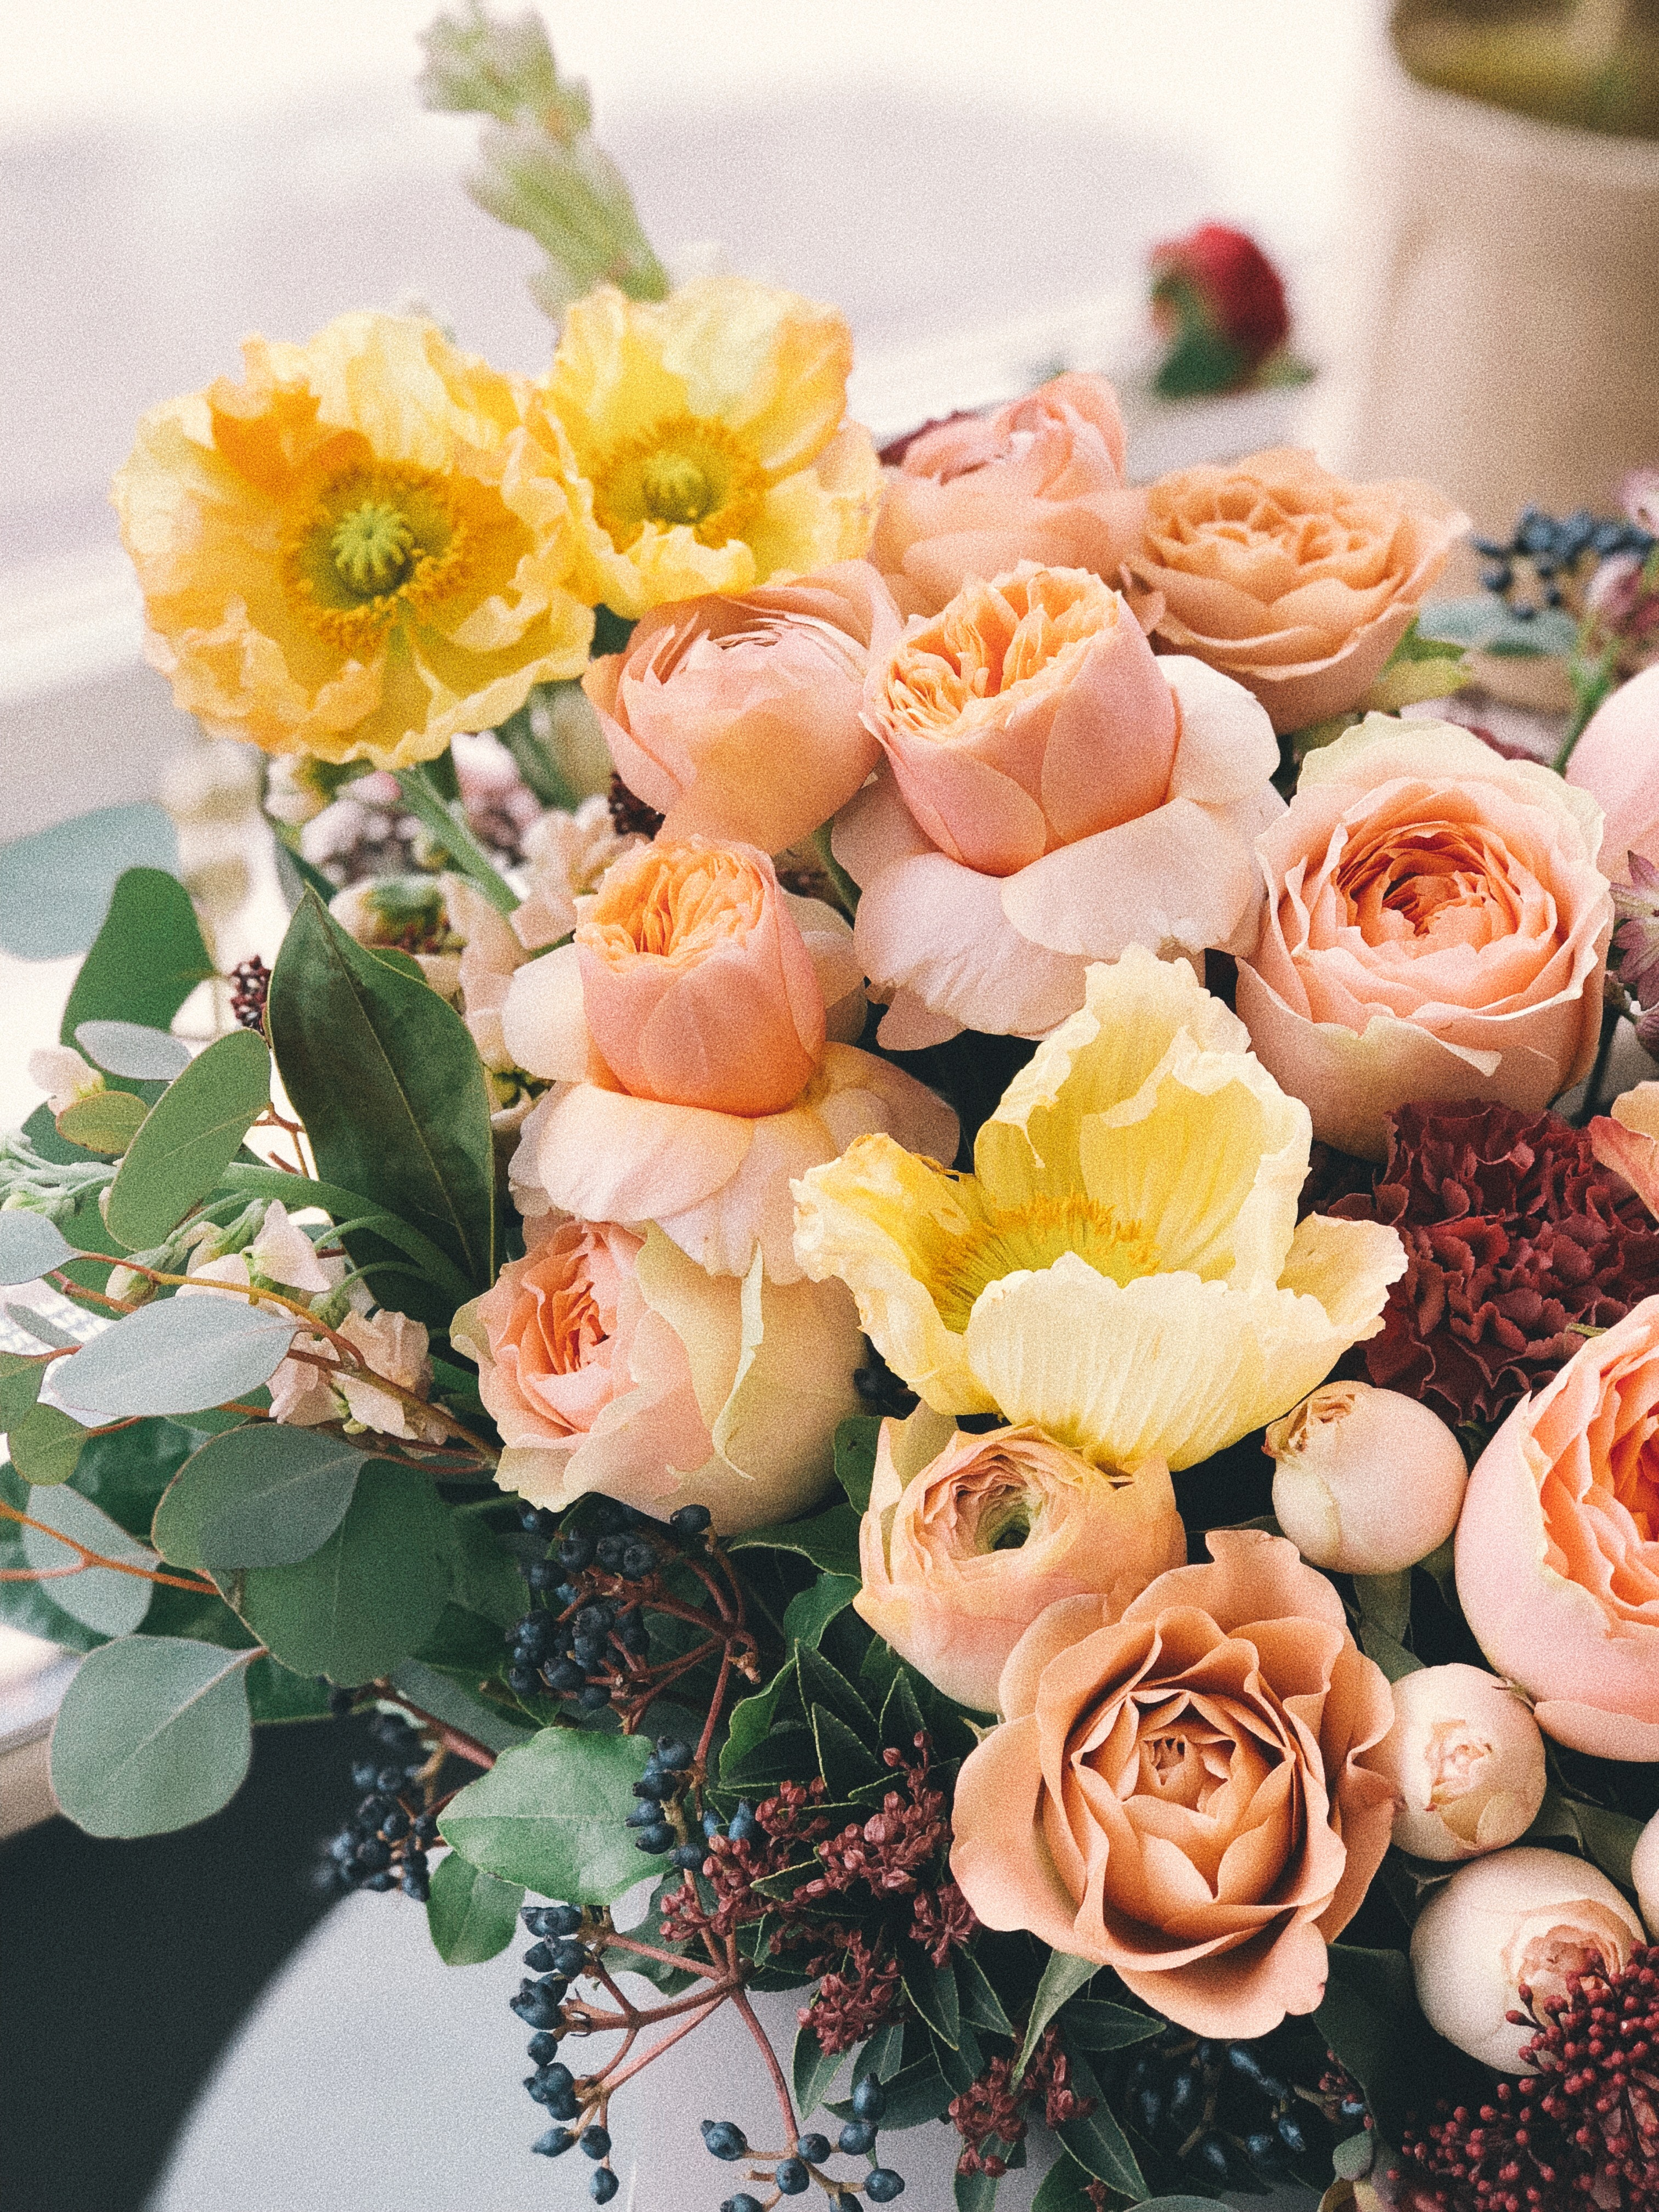
\includegraphics[height=0.8\textheight]{figures/bouquet.jpg}
      \end{figure}
    \end{column}
  \end{columns}

\end{frame}

\section{Maximum Likelihood Estimation}

\begin{frame}{Likelihood}
  \begin{align*}
    &P(\text{observed data}|\text{hypothesis})\\
    &P(\text{\flowers}|\text{\love})
  \end{align*}
\end{frame}

\begin{frame}{Maximum Likelihood}
  \begin{align*}
    P(\text{\flowers}|\text{\love}) &= 0.3 \\
    P(\text{\flowers}|\text{\emoji{broken-heart}}) &= 0.02
  \end{align*}
  \begin{itemize}[<2->]
    \item<2-> P(\text{\flowers}|\text{\love}) > P(\text{\flowers}|\text{\emoji{broken-heart}})
    \item<3-> \textbf{Conclusion:} \love
  \end{itemize}
\end{frame}

\begin{frame}{Maximum Likelihood}
  \begin{align*}
    P(\text{\flowers}|\text{\love}) &= 0.3 \\
    P(\text{\flowers}|\text{\emoji{orange-heart}}) &= 0.15 \\
    P(\text{\flowers}|\text{\emoji{yellow-heart}}) &= 0.075 \\
    P(\text{\flowers}|\text{\emoji{white-heart}}) &= 0.02 \\
  \end{align*}
\end{frame}

\begin{frame}
  \begin{align*}
    P(\text{\flowers}|\text{\love}) \neq P(\text{\love}|\text{\flowers})
  \end{align*}
\end{frame}

% \begin{frame}{MLE Example}
%   \begin{figure}[ht]
%     \centering
%     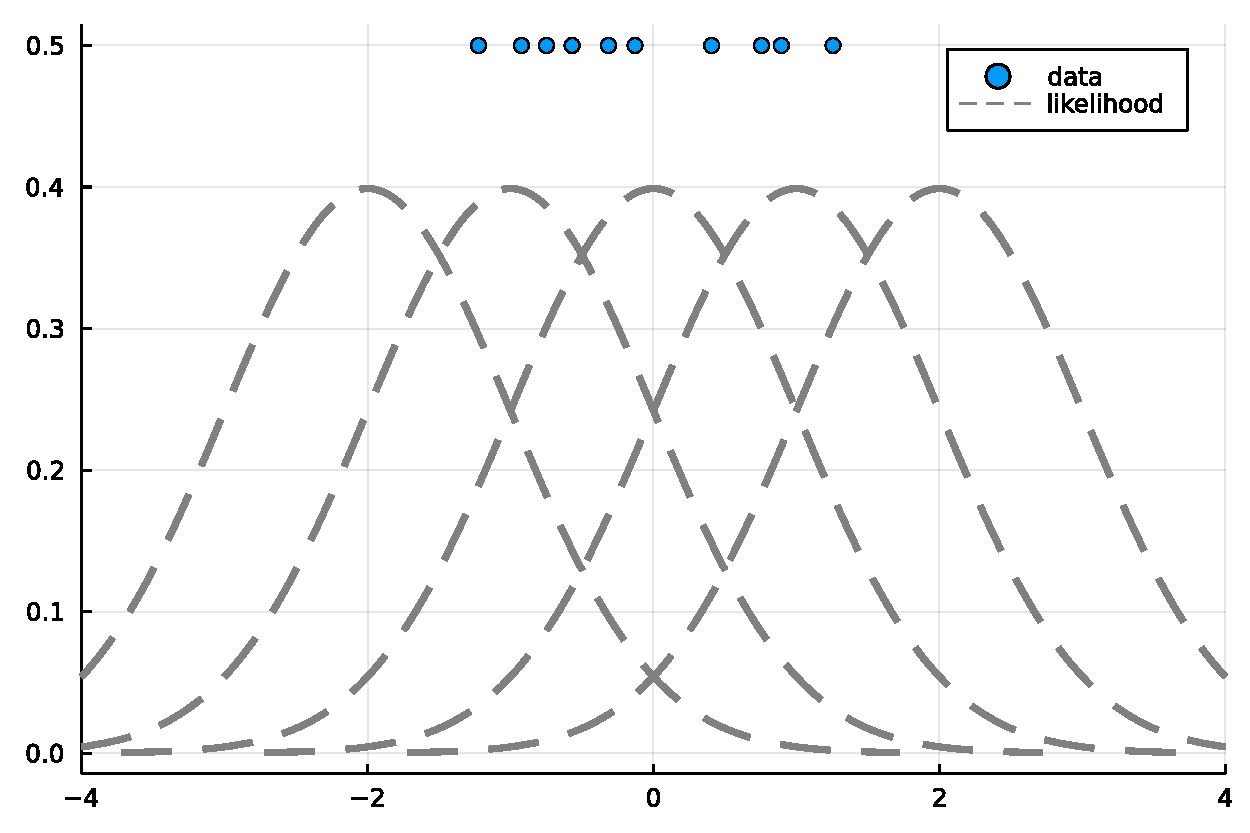
\includegraphics[width=0.8\textwidth]{figures/maximum_likelihood_estimation.pdf}
%   \end{figure}
% \end{frame}

\begin{frame}{Maximum Likelihood Estimation}
  \begin{itemize}
  \item Flexible!
  \item Needs some computational tricks (log-probabilities)
  \item Returns \emph{one single value}
  \item What if little data?
  \end{itemize}
\end{frame}

\section{Bayesian Statistics}

\begin{frame}
  \center
  What does a probability \textbf{mean}?
\end{frame}

\begin{frame}{Frequentist and Bayesian}
  \begin{block}{Frequentist}
    If I flip a coin for an \textbf{infinite number of times},
    half of the flips will turn heads.
  \end{block}

  \begin{block}{Bayesian}
    I do not know which side the coin I will see,
    so I say they have \textbf{equal chances}.
  \end{block}
\end{frame}

\begin{frame}{Bayes' rule}
  \begin{equation*}
    \tikz[baseline]{\node[anchor=base] (pab) {$P(B|A) \times P(A)$}}
    =
    \tikz[baseline]{\node[anchor=base] (pba) {$P(A|B) \times P(B)$}}
  \end{equation*}
  \begin{tikzpicture}[overlay, thick]
    \node<2->[above=of pab.north] (exp)  {$P(A \cap B)$};
    \node<2->[above=of pba.north] (exp1) {$P(B \cap A)$};
    % \node at (0, 1) {Other explanation};

    \draw<2-> (exp) -- (pab);
    \draw<2-> (exp1) -- (pba);
  \end{tikzpicture}
\end{frame}

\begin{frame}{Bayes' Rule}
  \begin{equation*}
    \tikz[baseline]{\node[anchor=base] (pab) {$P(\text{\love}) \times P(\text{\flowers}|\text{\love})$}}
    =
    \tikz[baseline]{\node[anchor=base] (pba) {$P(\text{\flowers}) \times P(\text{\love}|\text{\flowers})$}}
  \end{equation*}
  \begin{tikzpicture}[overlay, thick]
    \node<2->[above=of pab.north] (exp)  {$P(\text{\love} \cap \text{\flowers})$};
    \node<2->[above=of pba.north] (exp1) {$P(\text{\flowers} \cap \text{\love})$};
    % \node at (0, 1) {Other explanation};

    \draw<2-> (exp) -- (pab);
    \draw<2-> (exp1) -- (pba);
  \end{tikzpicture}
\end{frame}

\begin{frame}{Bayes' Rule}
\begin{equation*}
  P(\text{\love}|\text{\flowers})
  =
  \frac{P(\text{\love}) \times P(\text{\flowers}|\text{\love})} {P(\text{\flowers})}
\end{equation*}
\end{frame}


\newcommand{\markmath}[2]{\tikz[baseline]{\node[anchor=base] (#1) {$#2$}}}

\begin{frame}{Bayes' Rule}
\begin{equation*}
  \markmath{posterior}{P(\text{\love}|\text{\flowers})}
  =
  \frac{\markmath{prior}{P(\text{\love})} \times \markmath{likelihood}{P(\text{\flowers}|\text{\love})}} {\markmath{norm}{P(\text{\flowers})}}
\end{equation*}

\begin{tikzpicture}[overlay, thick,>=Stealth]
  \node<2->[above left=of prior] (priorlabel) {Prior};
  \node<3->[above right=of likelihood] (liklabel) {Likelihood};
  \node<4->[left=of posterior] (postlabel) {Posterior};
  \node<5->[below=of norm] (normlabel) {Normalization};


  \draw<2->[->] (priorlabel) -- (prior);
  \draw<3->[->] (liklabel) -- (likelihood);
  \draw<4->[->] (postlabel) -- (posterior.west);
  \draw<5->[->] (normlabel) -- (norm);
\end{tikzpicture}
\end{frame}

\begin{frame}{Bayes' Rule}
  \begin{equation*}
    P(\text{\love}|\text{\flowers}) \propto P(\text{\love}) \times P(\text{\flowers}|\text{\love})
  \end{equation*}
\end{frame}

\begin{frame}
  \begin{block}{Bayesian Statistics}
    \begin{enumerate}
    \item Express your \emph{beliefs} in math (priors)
    \item Test them against the evidence (likelihood)
    \item Update your beliefs (posteriors)
    \end{enumerate}
  \end{block}

  % \begin{centering}
  %   <2->{Distributions in, Distributions out}
  % \end{centering}
\end{frame}

\begin{frame}
  \begin{itemize}
  \item Flexible!
  \item Needs some computational tricks too (lots!)
  \item Returns distributions
  \item Works with little data
  \end{itemize}
\end{frame}

\section{Comparing two means}

\begin{frame}
  \begin{figure}[ht]
    \centering
    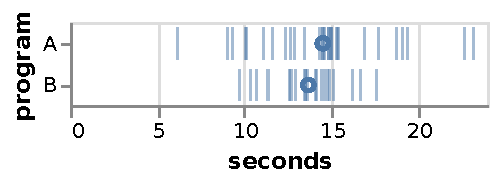
\includegraphics[width=0.8\textwidth]{figures/samples_a_b.pdf}
    % \caption{\label{fig:label} }
  \end{figure}
\end{frame}

\begin{frame}
\begin{figure}[ht]
  \centering
  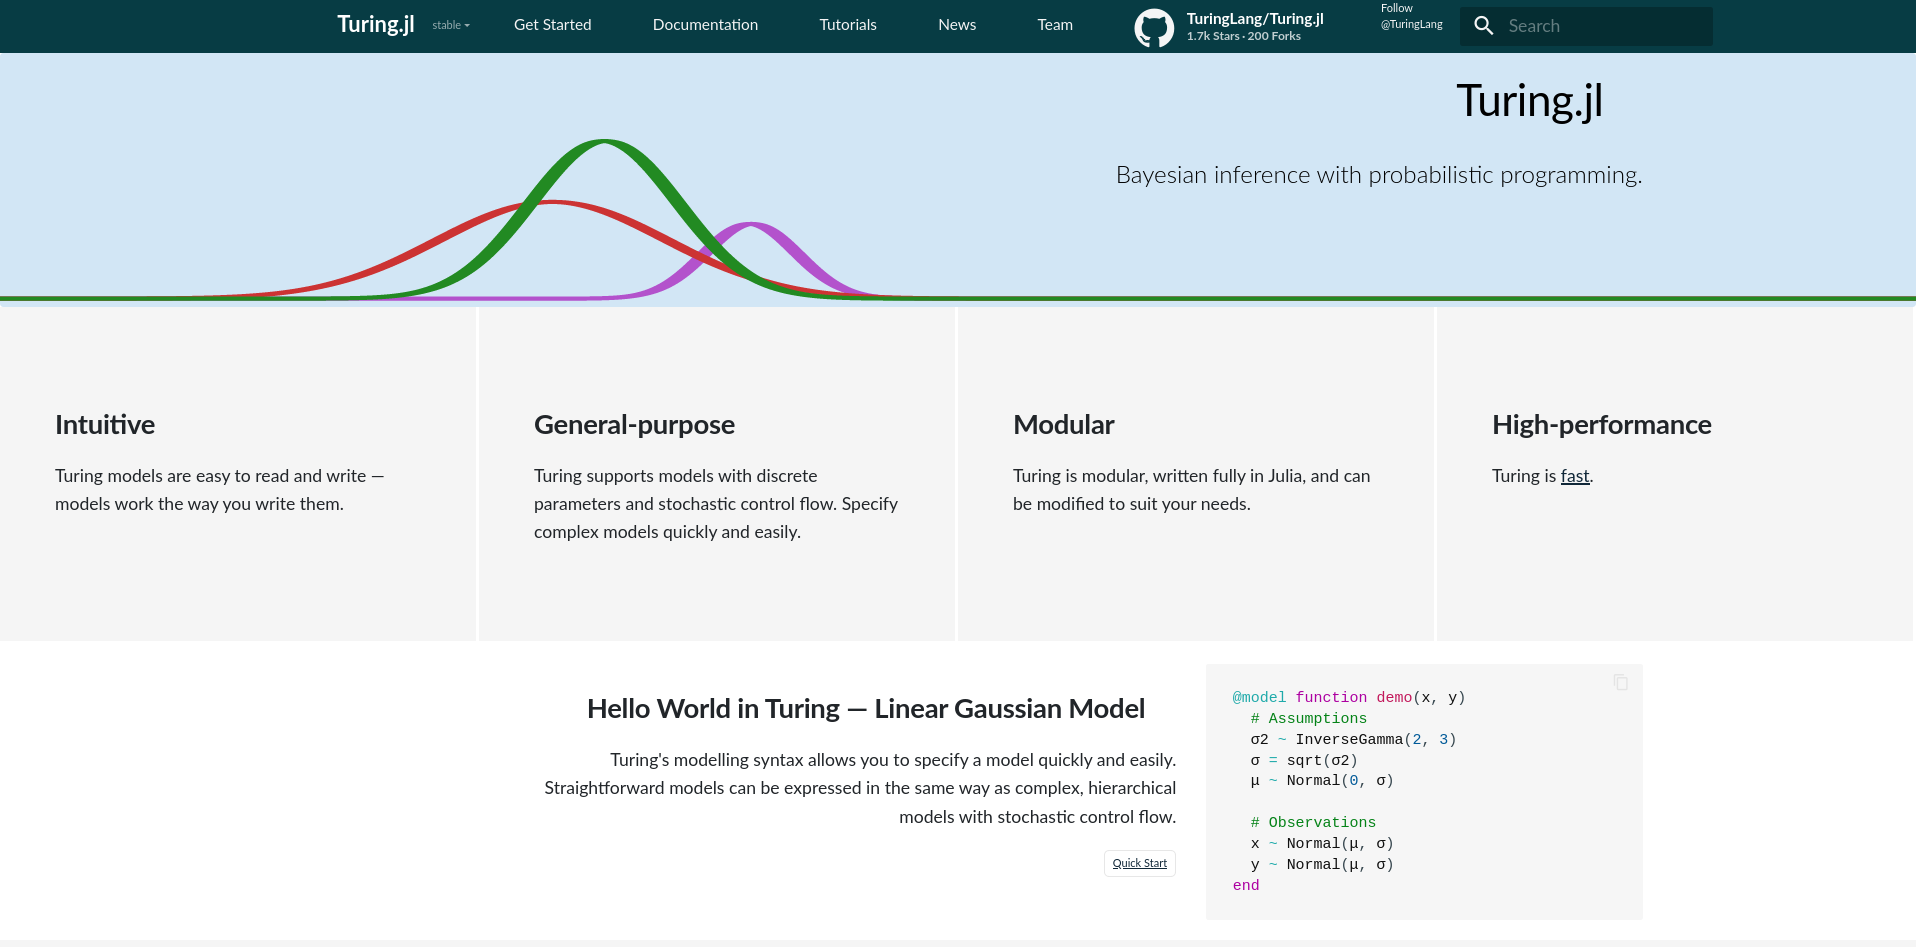
\includegraphics[width=0.9\textwidth]{figures/turingjl.png}
\end{figure}
\end{frame}

% We use the notation from McElreath p.32
% Paramters and observed parameter
\newcommand{\parameter}[1]{\textcolor{orange}{#1}}
\newcommand{\observed}[1]{\textcolor{cyan}{#1}}

\newcommand{\normal}[1]{\text{Normal}(#1)}
\newcommand{\exponential}[1]{\text{Exponential}(#1)}

\begin{frame}{Mathematical Model}
  \begin{align*}
    \observed{A_i} &\sim \normal{\parameter{\mu_A}, \parameter{\sigma_A}}\\
    \observed{B_i} &\sim \normal{\parameter{\mu_B}, \parameter{\sigma_B}}\\
    \parameter{\mu_A} &\sim \normal{10.0, 5.0}\\
    \parameter{\mu_B} &\sim \normal{10.0, 5.0}\\
    \parameter{\sigma_A} &\sim \exponential{1.0}\\
    \parameter{\sigma_B} &\sim \exponential{1.0}\\
  \end{align*}

  \begin{itemize}
  \item \parameter{x} Parameter
  \item \observed{x} Observed
  \end{itemize}
\end{frame}

\begin{frame}
  \begin{columns}
    \begin{column}{0.5\textwidth}
      \center
      \begin{tikzpicture}[>=Stealth]
        \draw[thick] (0, 2) -- (0, -2);
        \fill (-2, 0) circle[radius=2pt] node[above] {fixed};

        \draw (-2, 0) -- (0, 0);

        \draw (0,0) -- (2,0) circle[radius=2pt] ;
        \draw (0,0) -- (2,0.5) circle[radius=2pt] ;
        \draw (0,0) -- (2,-0.4) circle[radius=2pt] ;
        \draw (0,0) -- (2,1.2) circle[radius=2pt] ;
        \draw (0,0) -- (2,-1.3) circle[radius=2pt] ;

        \draw[decorate, decoration={coil, aspect=0}] (1.75, 2) -- (1.75,-2);
        \draw[decorate, decoration={coil, aspect=0}] (2.25, 2) -- (2.25,-2);

        \draw[->,thick] (-2, -3) -- node[midway,above] {Simulation} (2, -3);
      \end{tikzpicture}
    \end{column}
    \begin{column}{0.5\textwidth}
      \center
      \begin{tikzpicture}[>=Stealth]
        \draw[thick] (0, 2) -- (0, -2);
        \draw(-2, 0) circle[radius=2pt];
        \draw(-2, 0.1) circle[radius=2pt];
        \draw(-2, 0.07) circle[radius=2pt];
        \draw(-2, -0.03) circle[radius=2pt];
        \draw(-2, -0.12) circle[radius=2pt];

        \draw (-2, 0) -- (0, 0);

        \draw[decorate, decoration={coil, aspect=0}] (-1.75, 2) -- (-1.75,-2);
        \draw[decorate, decoration={coil, aspect=0}] (-2.25, 2) -- (-2.25,-2);

        \draw[fill=black] (2,0) circle[radius=2pt] -- (0,0);
        \draw[fill=black] (2,0.5) circle[radius=2pt] -- (0,0);
        \draw[fill=black] (2,-0.4) circle[radius=2pt] -- (0,0);
        \draw[fill=black] (2,1.2) circle[radius=2pt] -- (0,0);
        \draw[fill=black] (2,-1.3) circle[radius=2pt] node[below] {fixed} -- (0,0);


        \draw[->,thick] (2, -3) -- node[midway,above] {Inference} (-2, -3);
      \end{tikzpicture}
    \end{column}
  \end{columns}
\end{frame}





\begin{frame}[fragile]
    % mu_a = 15.0
    % mu_b = 13.0

    % sigma_a = 4.0
    % sigma_b = 2.0
    \begin{minted}[autogobble,fontsize=\footnotesize]{julia}
    function generate_samples(mean_a, mean_b, stdev_a, stdev_b)
        n_a = 30
        n_b = 20

        As = zeros(n_a)
        Bs = zeros(n_b)
        for i in 1:n_a
            As[i] = rand(Normal(mean_a, stdev_a))
        end

        for i in 1:n_b
            Bs[i] = rand(Normal(mean_b, stdev_b))
        end

        return (As,Bs)
    end
    \end{minted}
\end{frame}

\begin{frame}[fragile]
  \begin{minted}{julia}
@model function means_model(As, Bs)
    # Priors
    mean_a ~ Normal(10.0, 5.0)
    mean_b ~ Normal(10.0, 5.0)

    stdev_a ~ Exponential(1.0)
    stdev_b ~ Exponential(1.0)

    # Likelihood
    for i in eachindex(As)
        As[i] ~ Normal(mean_a, stdev_a)
    end

    for i in eachindex(Bs)
        Bs[i] ~ Normal(mean_b, stdev_b)
    end
end
  \end{minted}
\end{frame}

\begin{frame}[fragile]
  \begin{minted}[autogobble]{julia}
    # Create model (pass the data to it)
    model = means_model(samples_a, samples_b)

    # Run bayesian inference
    chain = sample(model, NUTS(0.65), 5000)

    # Get posterior samples for a variable in model
    chain[:mean_a]
  \end{minted}
\end{frame}

\begin{frame}
  \begin{figure}[ht]
    \centering
    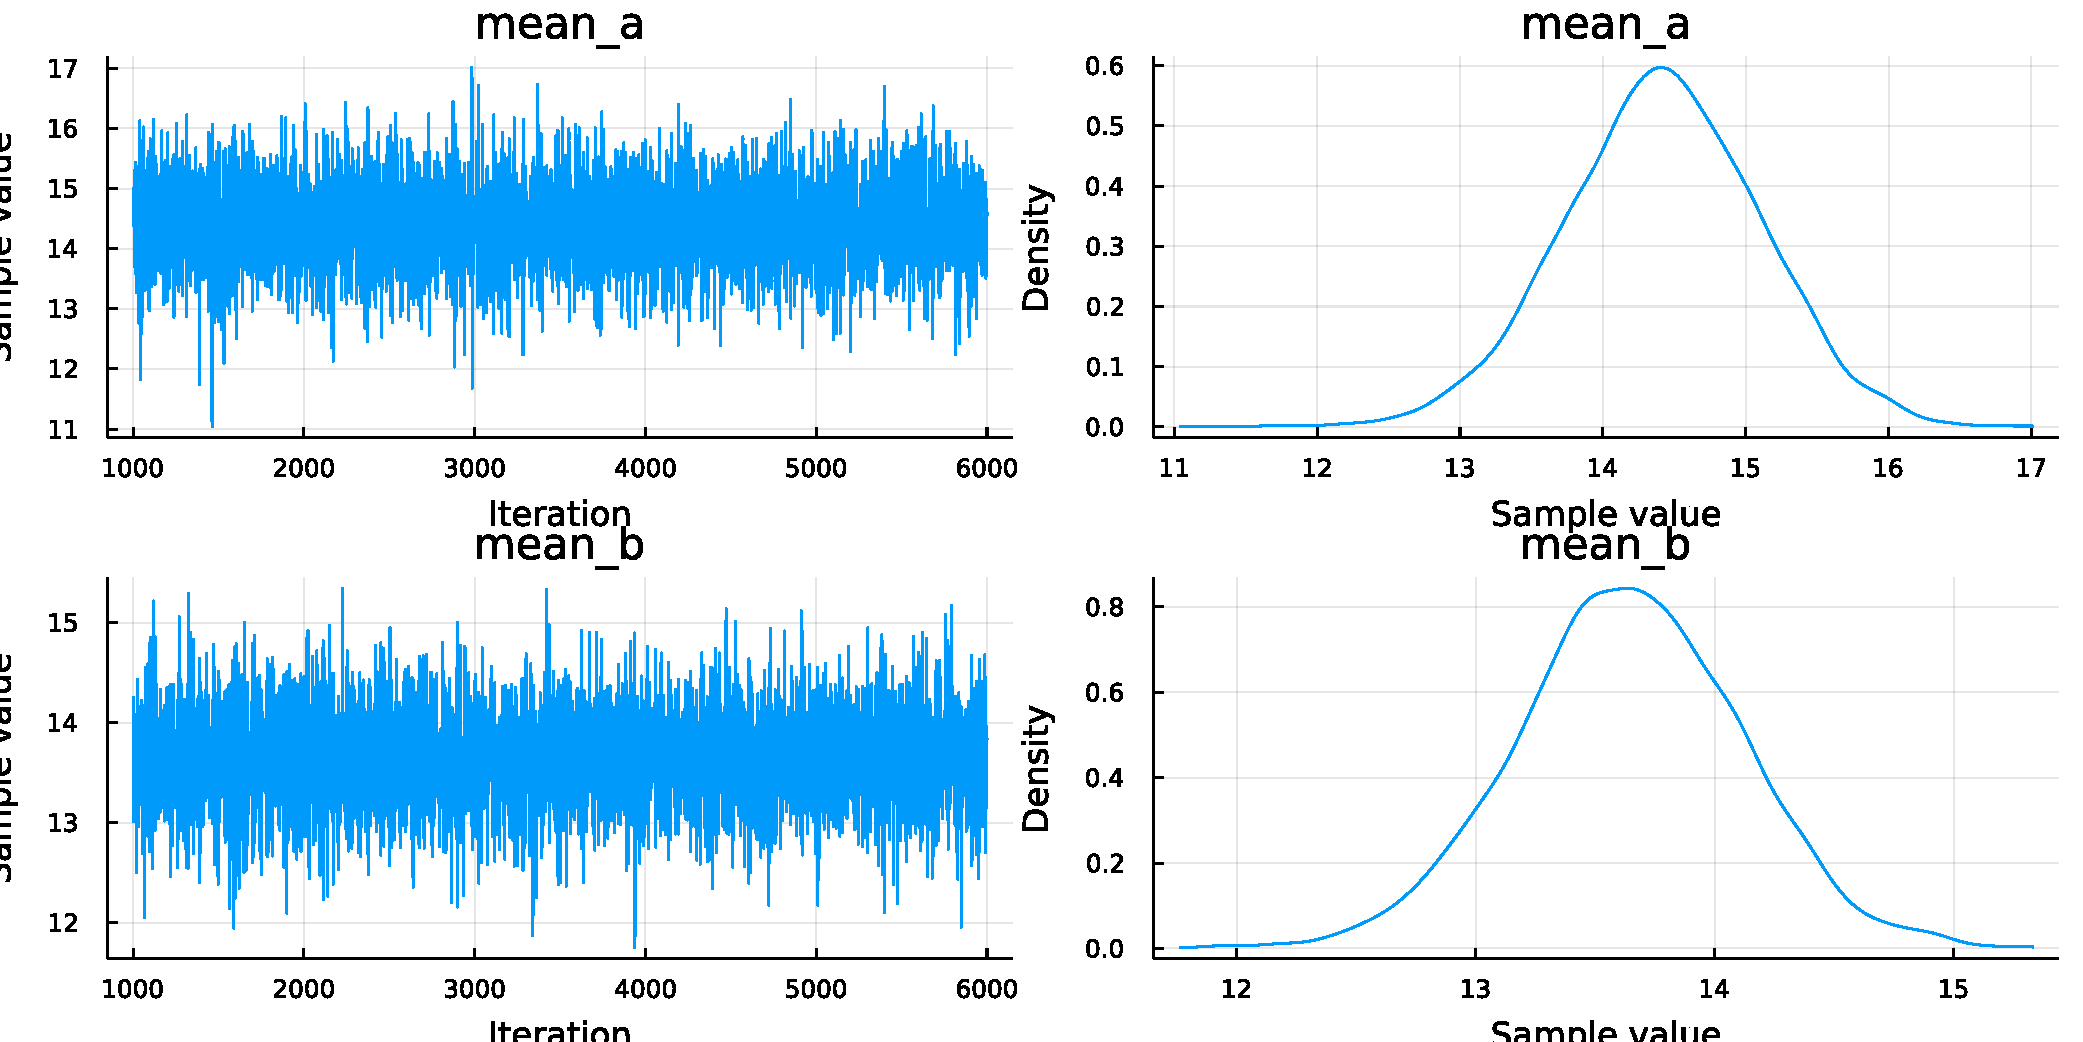
\includegraphics[height=0.7\textheight]{figures/chain_mean.pdf}
  \end{figure}
\end{frame}

\begin{frame}
  \begin{figure}[ht]
    \centering
    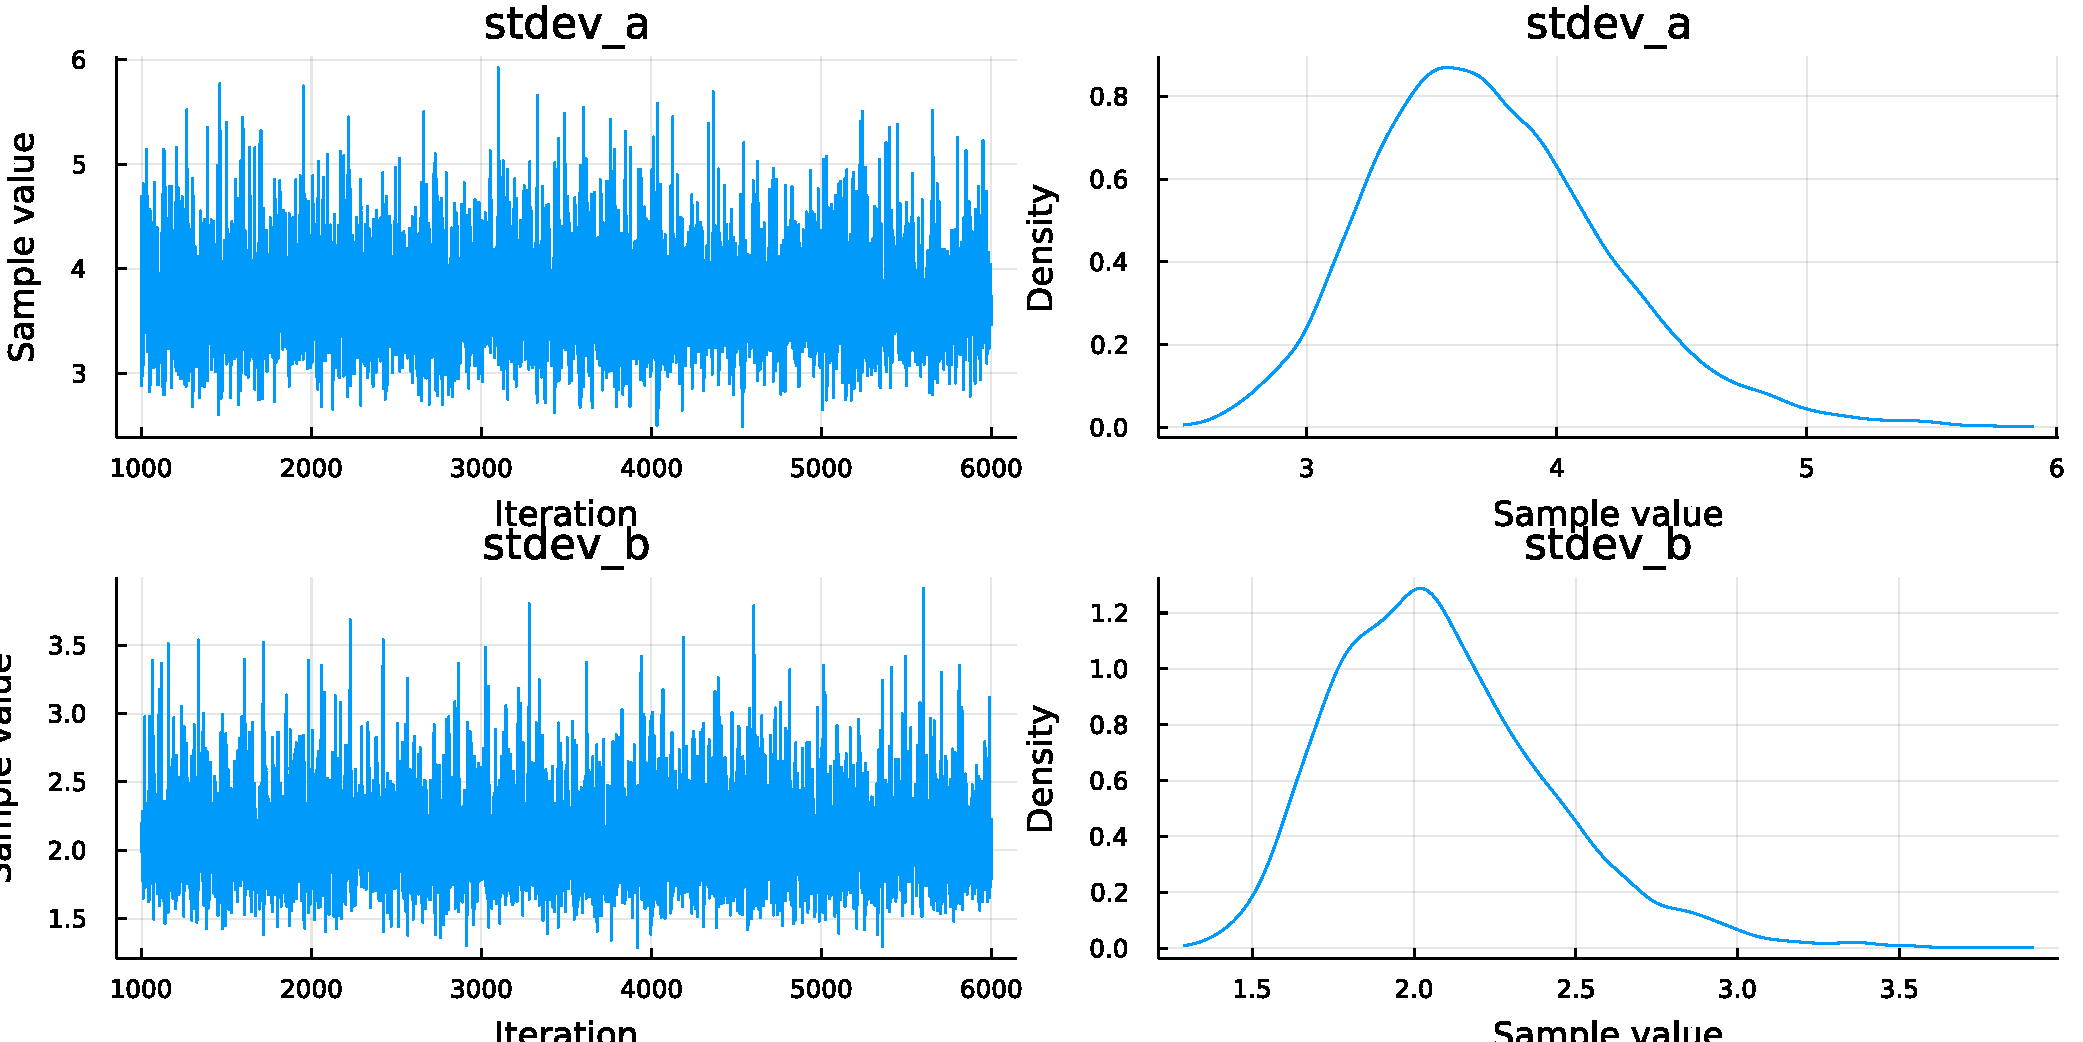
\includegraphics[height=0.7\textheight]{figures/chain_stdev.pdf}
  \end{figure}
\end{frame}

\begin{frame}
  \begin{figure}[ht]
    \centering
    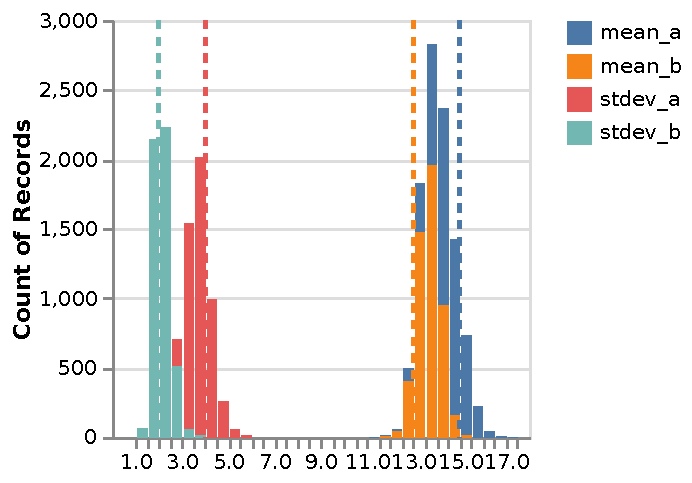
\includegraphics[width=0.7\textwidth]{figures/plot_a_b_parameters.pdf}
    % \caption{\label{fig:label} }
  \end{figure}
\end{frame}

\begin{frame}[fragile]
  \begin{minted}[autogobble]{julia}
    diff = chain[:mean_b] - chain[:mean_a]
  \end{minted}

  \begin{figure}[ht]
    \centering
    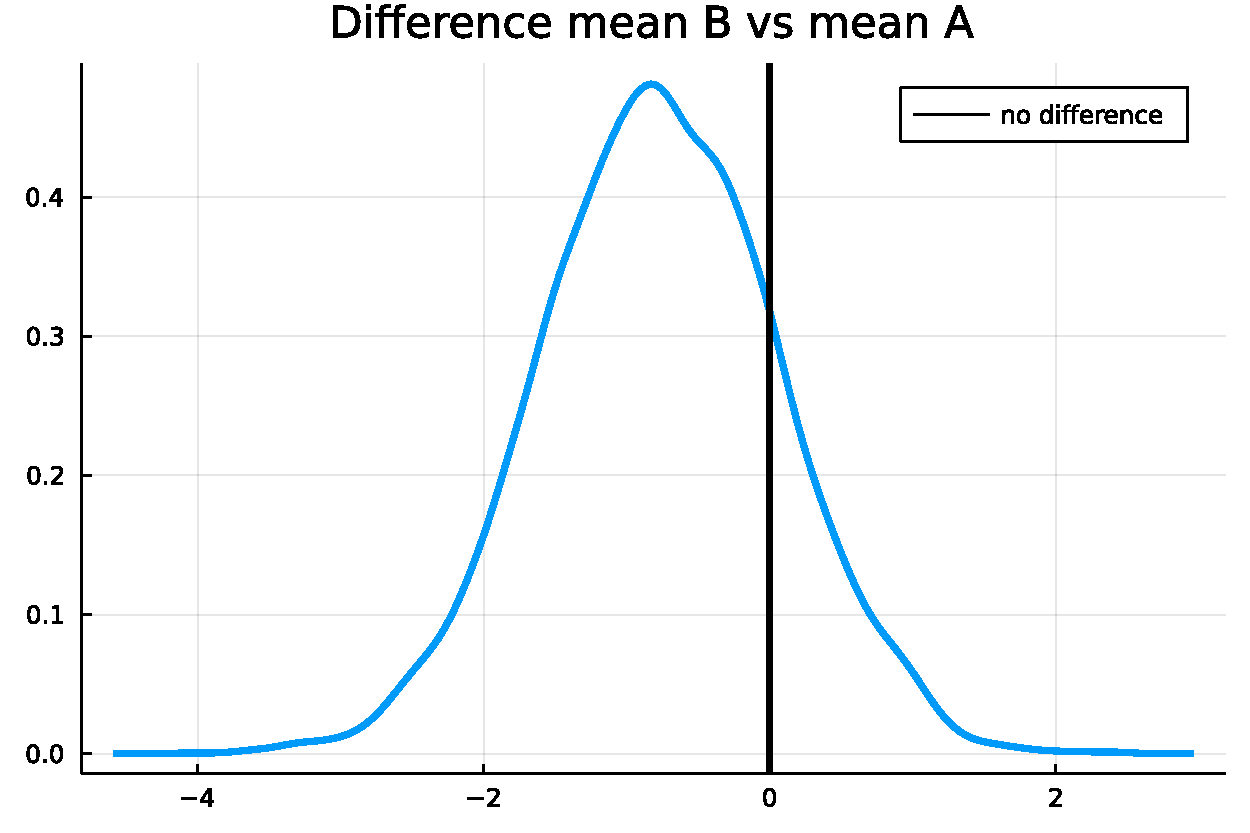
\includegraphics[width=0.6\textwidth]{figures/plot_difference_a_b.pdf}
  \end{figure}
\end{frame}

\section{Posterior predictive simulation}

\begin{frame}
  \huge
  \center
  Predictions return \emph{distributions} too!
\end{frame}

\begin{frame}
  \begin{itemize}
  \item \textbf{Prediction:} You know the inputs and the function, but not the outputs
  \item \textbf{Inference:} You know the outputs and the function, but not the inputs
  \item \textbf{Learning:} You know the inputs and the outputs, but not the function
  \end{itemize}

  \begin{block}{Posterior predictive simulation}
    Make \textbf{predictions} with some uncertain inputs
  \end{block}
\end{frame}

\begin{frame}[fragile]
    \begin{minted}[autogobble,fontsize=\footnotesize]{julia}
    function generate_samples(mean_a, mean_b, stdev_a, stdev_b)
        n_a = 30
        n_b = 20

        As = zeros(n_a)
        Bs = zeros(n_b)
        for i in 1:n_a
            As[i] = rand(Normal(mean_a, stdev_a))
        end

        for i in 1:n_b
            Bs[i] = rand(Normal(mean_b, stdev_b))
        end

        return (As,Bs)
    end
    \end{minted}
\end{frame}

\begin{frame}
\begin{figure}[ht]
  \centering
  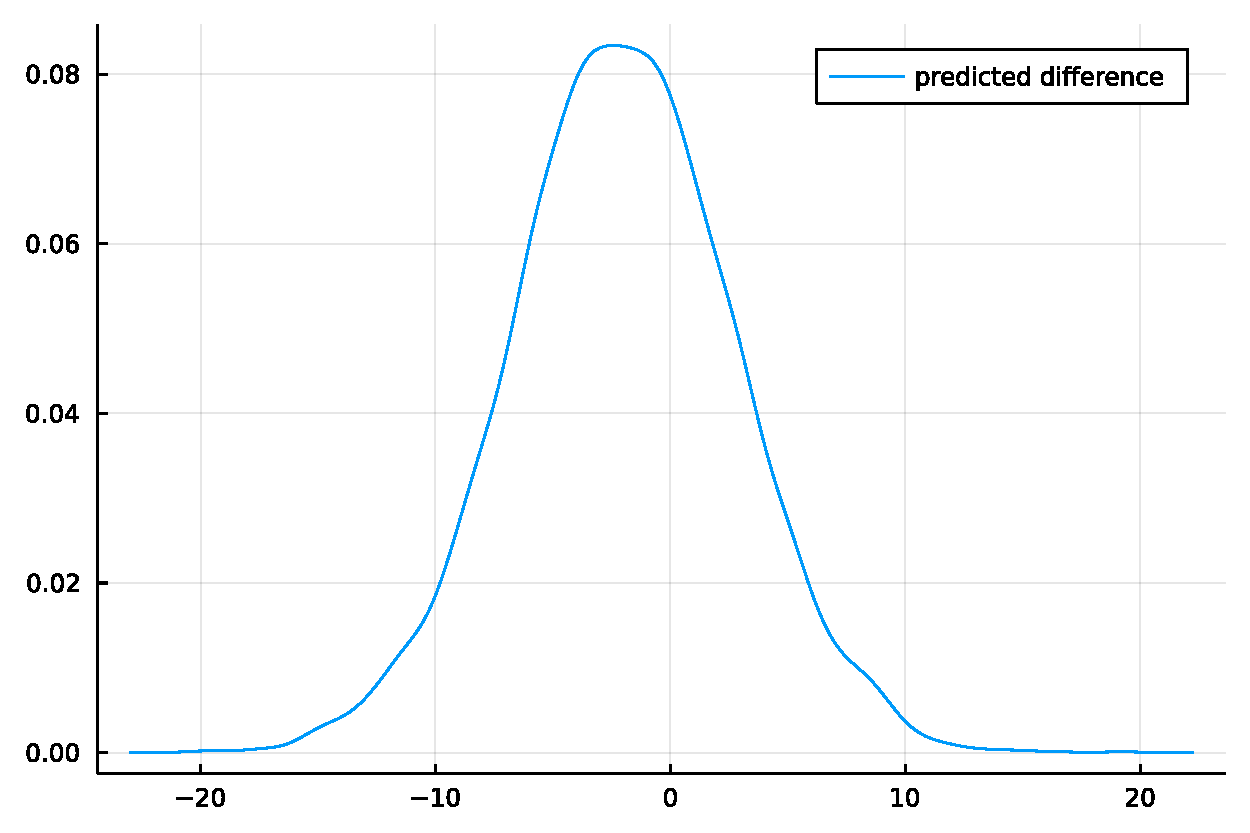
\includegraphics[width=0.7\textwidth]{figures/predicted_difference_a_b.pdf}
\end{figure}
\end{frame}

\section{Linear regression}

\begin{frame}
\begin{figure}[ht]
  \centering
  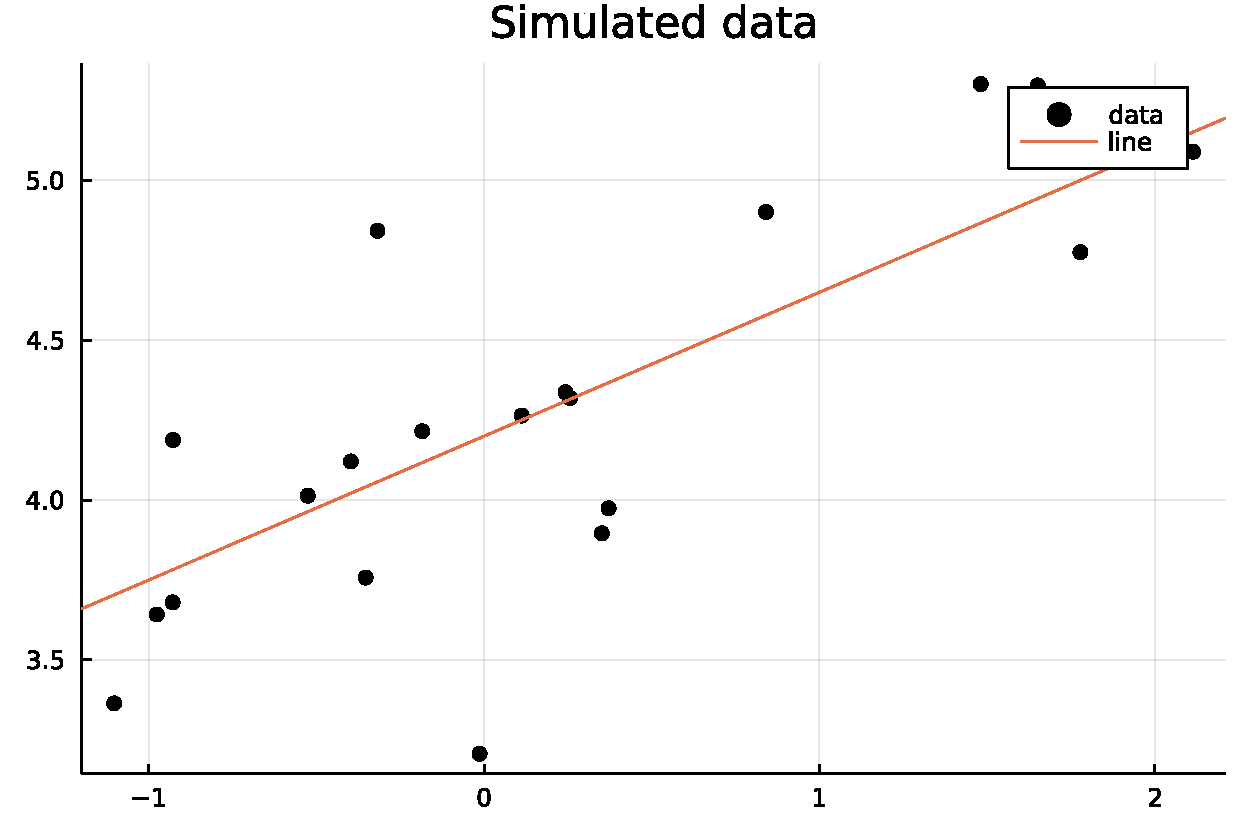
\includegraphics[width=0.8\textwidth]{figures/linear_data.pdf}
  \caption{\label{fig:label} Simulated data}
\end{figure}
\end{frame}

\begin{frame}
  \begin{block}{Why is linear regression useful?}
    \begin{itemize}
    \item simple model, but easy to extend
    \item shows positive/negative associations
    \item interpretable
    \end{itemize}
  \end{block}
\end{frame}

\begin{frame}
  \begin{align*}
    \observed{y_i} &\sim \normal{\mu_i, \parameter{\sigma}}\\
    \mu_i &= \parameter{\alpha} \observed{x_i} + \parameter{\beta}\\
    \parameter{\alpha} &\sim \normal{0,1}\\
    \parameter{\beta} &\sim \normal{0, 1}\\
    \parameter{\sigma} &\sim \exponential{0.2}\\
  \end{align*}

  \begin{itemize}
  \item \parameter{x} Parameter
  \item \observed{x} Observed
  \end{itemize}
\end{frame}

\begin{frame}
  \begin{figure}[ht]
    \centering
    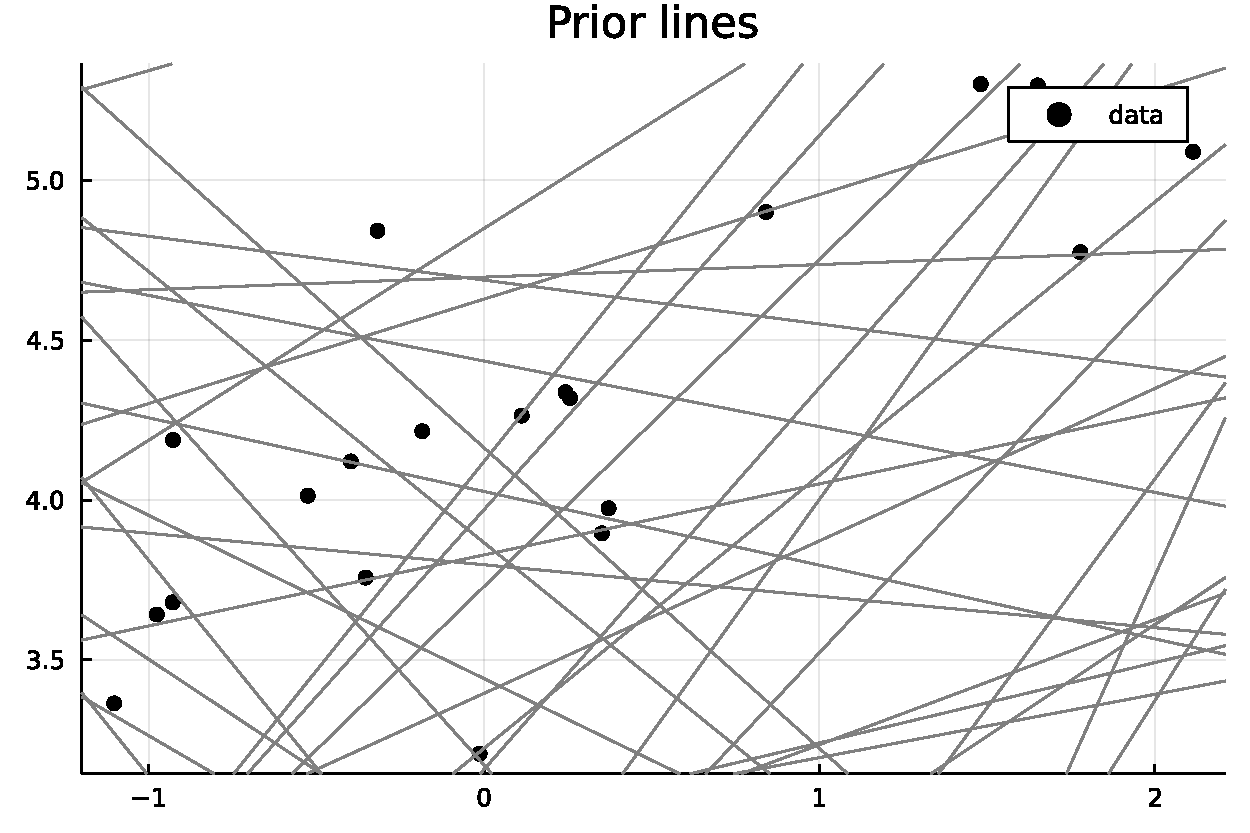
\includegraphics[width=0.8\textwidth]{figures/linear_prior_lines.pdf}
  \end{figure}
\end{frame}

\begin{frame}
  \begin{figure}[ht]
    \centering
    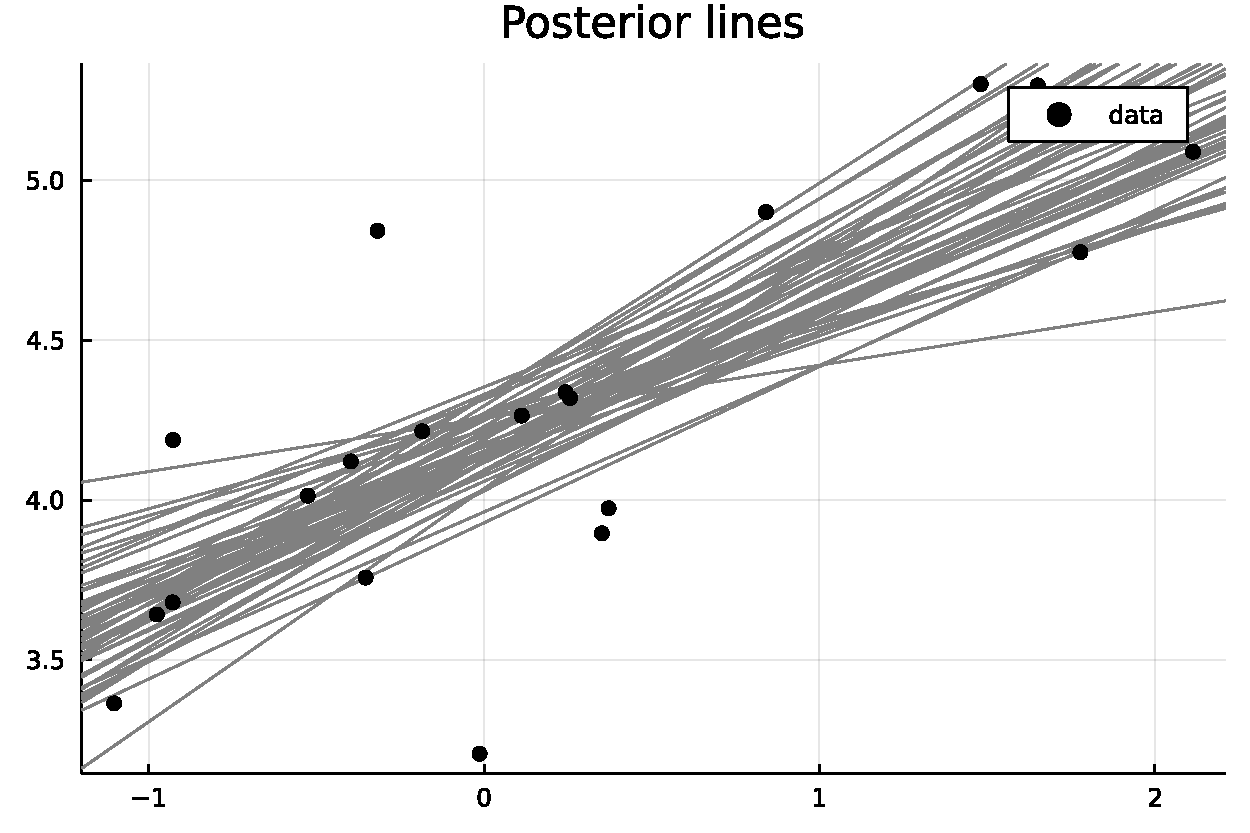
\includegraphics[width=0.8\textwidth]{figures/posterior_lines.pdf}
  \end{figure}
\end{frame}

\begin{frame}
\begin{figure}[ht]
  \centering
  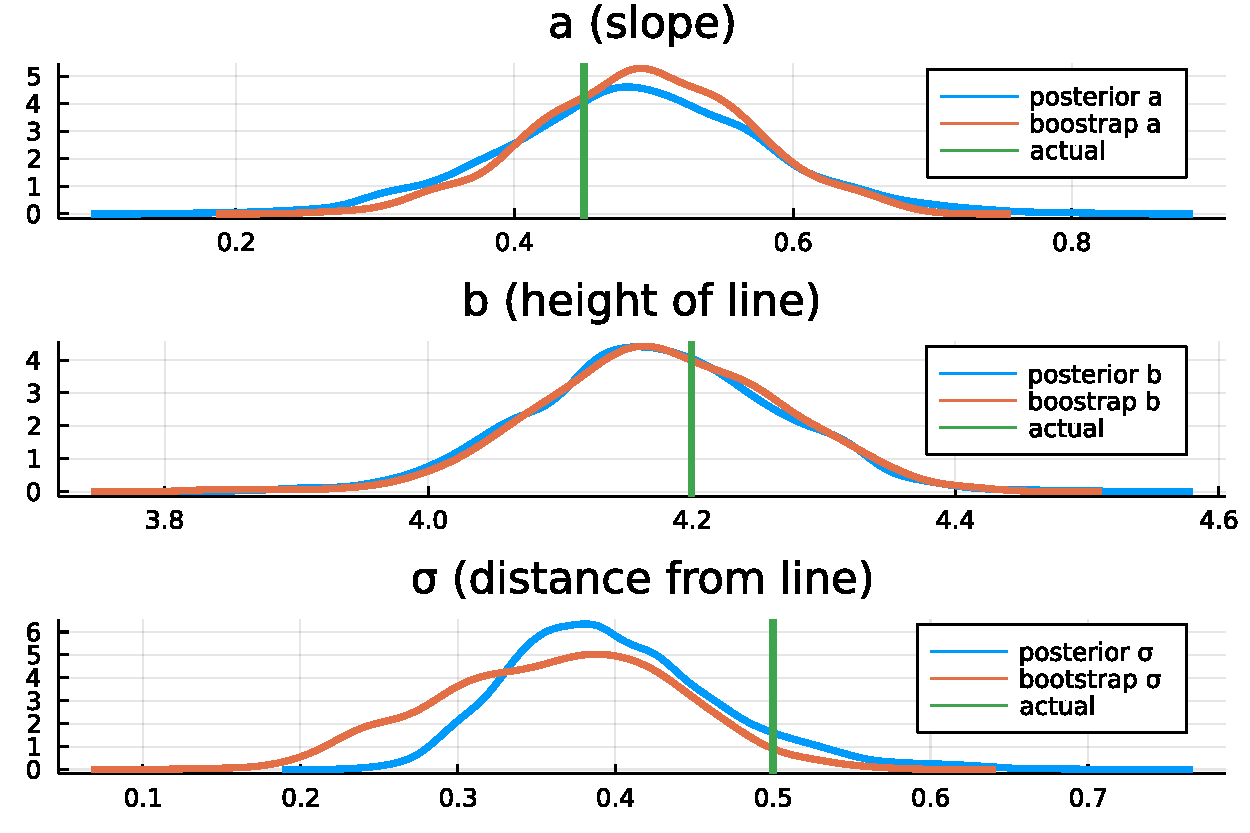
\includegraphics[width=0.8\textwidth]{figures/posterior_parameters.pdf}
\end{figure}
\end{frame}

\begin{frame}
\begin{figure}[ht]
  \centering
  \begin{tikzpicture}[thick,>=Stealth]
    \node (priors) at (-1, 1) {Prior(s)};
    \node (posteriors) at (0,0) {Posterior(s)};
    \node (likelihood) at (1,1) {Likelihood};
    \node (data) at (-1,2) {Observations};
    \node (structure) at (2,2) {Structure};

    \draw[->] (priors) -- (posteriors);
    \draw[->] (likelihood) -- (posteriors);
    \draw[->] (data) -- (likelihood);
    \draw[->] (structure) -- (likelihood);
  \end{tikzpicture}
\end{figure}
\end{frame}

\section{Posterior predictive simulation}

\begin{frame}
  \huge
  \center
  Predictions return \emph{distributions} too!
\end{frame}

\begin{frame}
  \begin{figure}[ht]
    \centering
    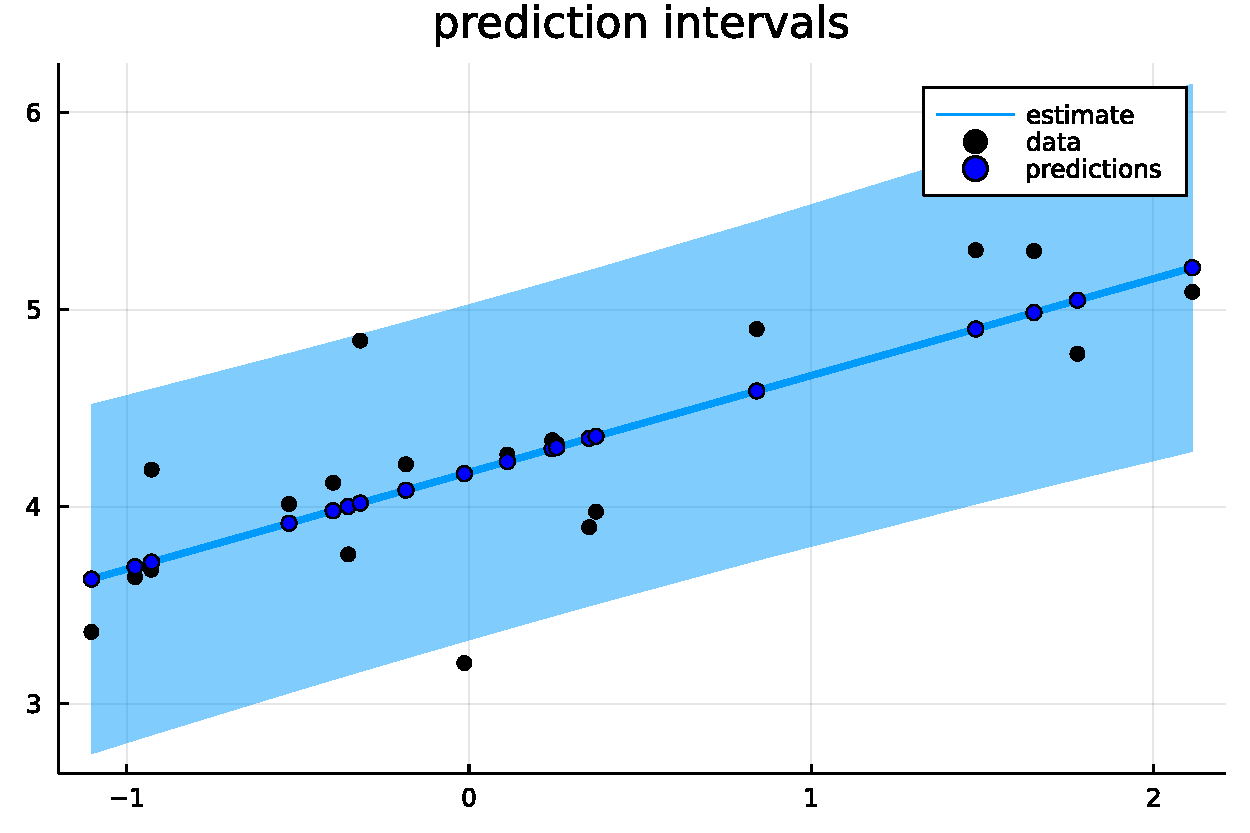
\includegraphics[width=0.8\textwidth]{figures/linear_prediction_interval.pdf}
  \end{figure}
\end{frame}

\begin{frame}
\begin{figure}[ht]
  \centering
  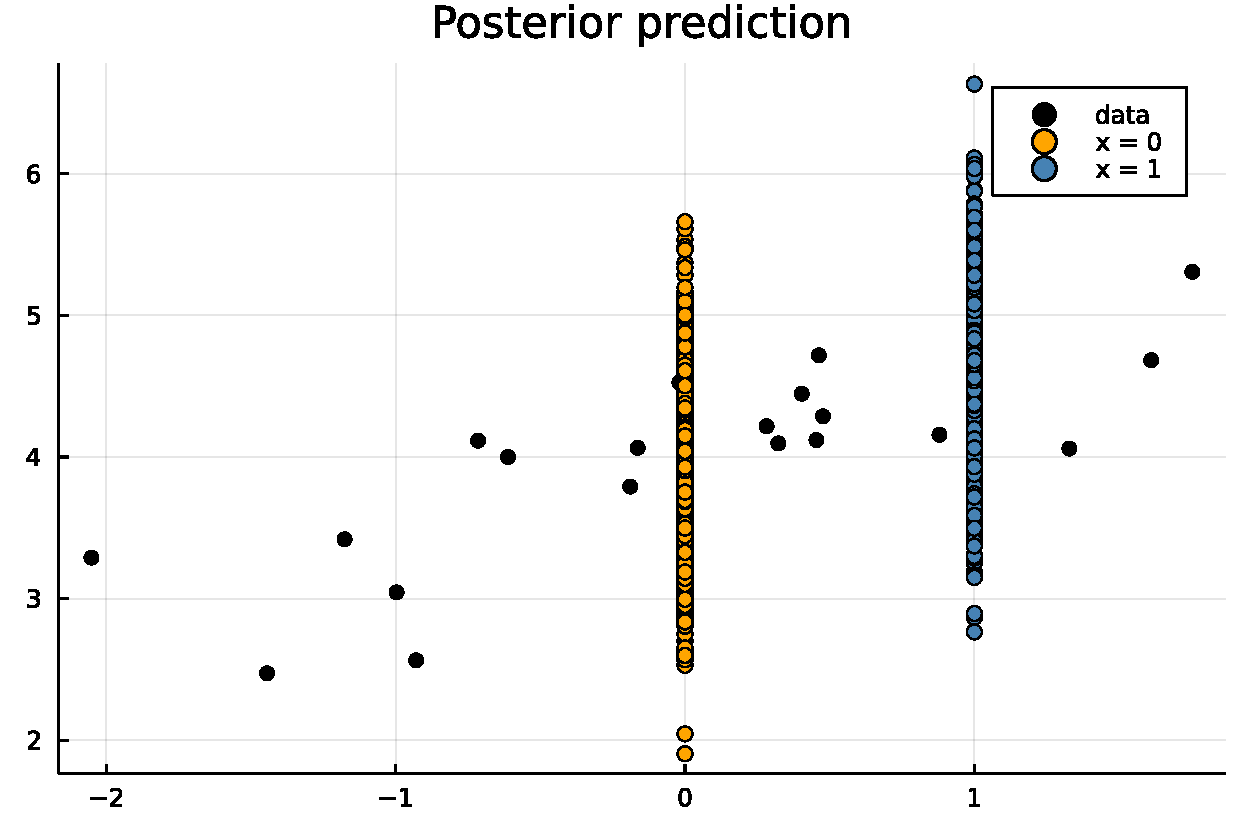
\includegraphics[width=0.8\textwidth]{figures/predictions.pdf}
\end{figure}
\end{frame}

\begin{frame}
\begin{figure}[ht]
  \centering
  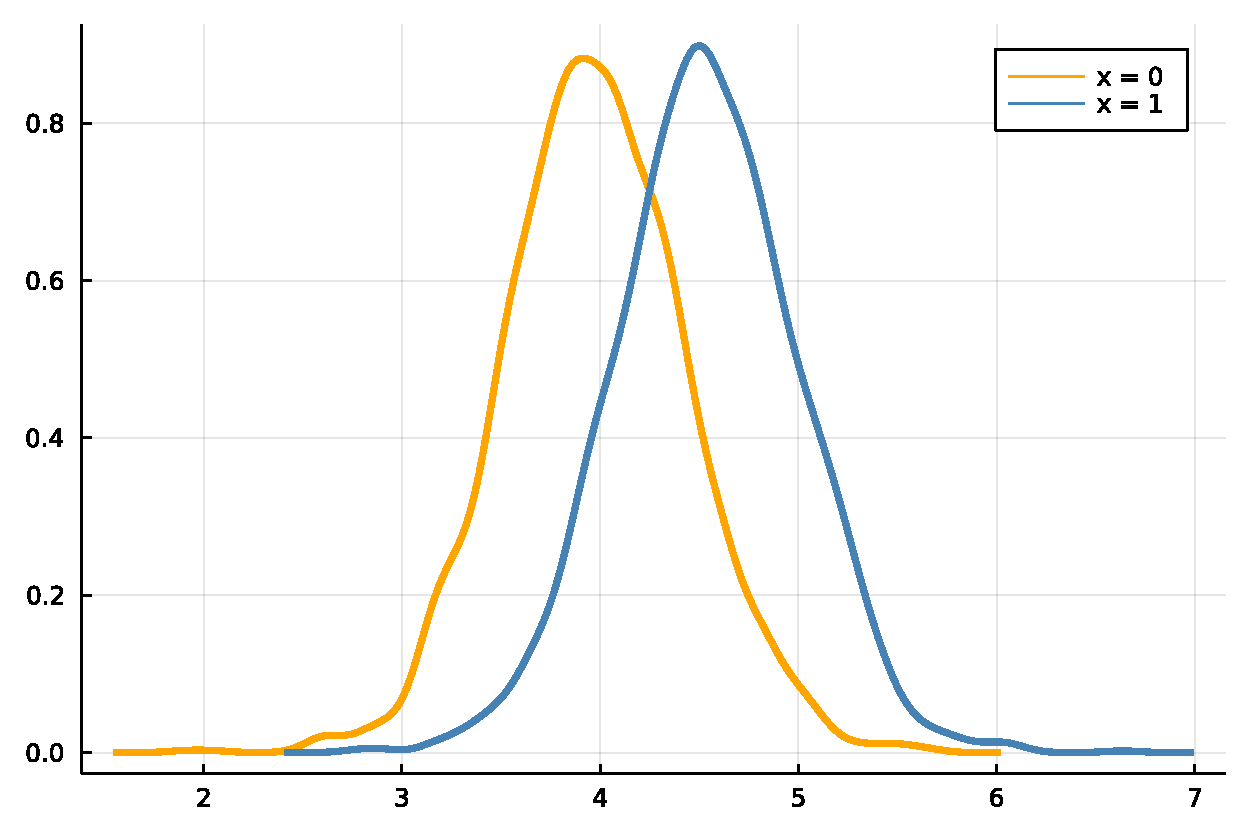
\includegraphics[width=0.8\textwidth]{figures/prediction_distrubtions.pdf}
\end{figure}
\end{frame}

\begin{frame}
\begin{figure}[ht]
  \centering
  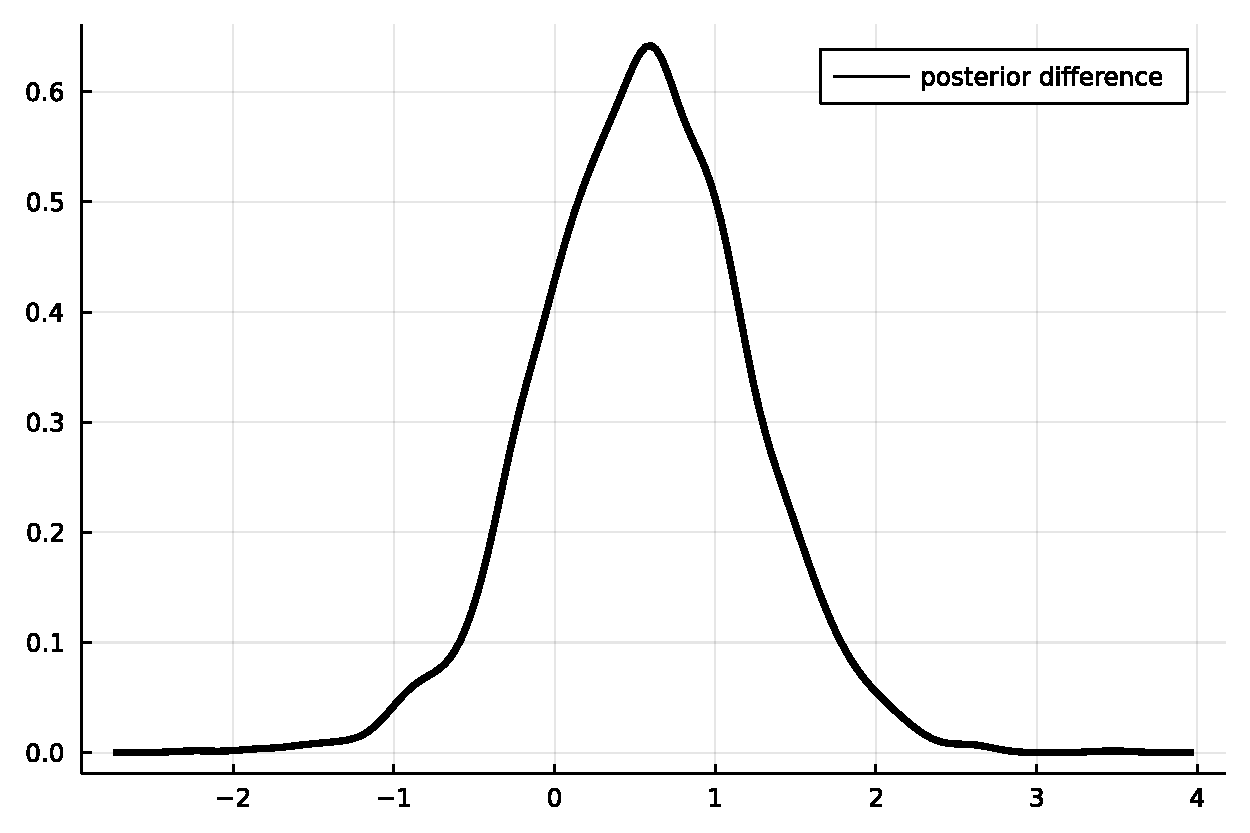
\includegraphics[width=0.8\textwidth]{figures/prediction_difference.pdf}
\end{figure}
\end{frame}

\section{Interactions}

\begin{frame}
  \begin{block}{Examples of interactions}
    \begin{itemize}
    \item Plants need both \textbf{light} and \textbf{water} to grow.
    \item To have sweet coffee you need to \textbf{add sugar} and \textbf{stir} the coffee.
    \item \textbf{Some optimizations} only work on \textbf{some CPUs}.
    \end{itemize}
  \end{block}
\end{frame}

\begin{frame}
  \begin{figure}[ht]
    \centering
    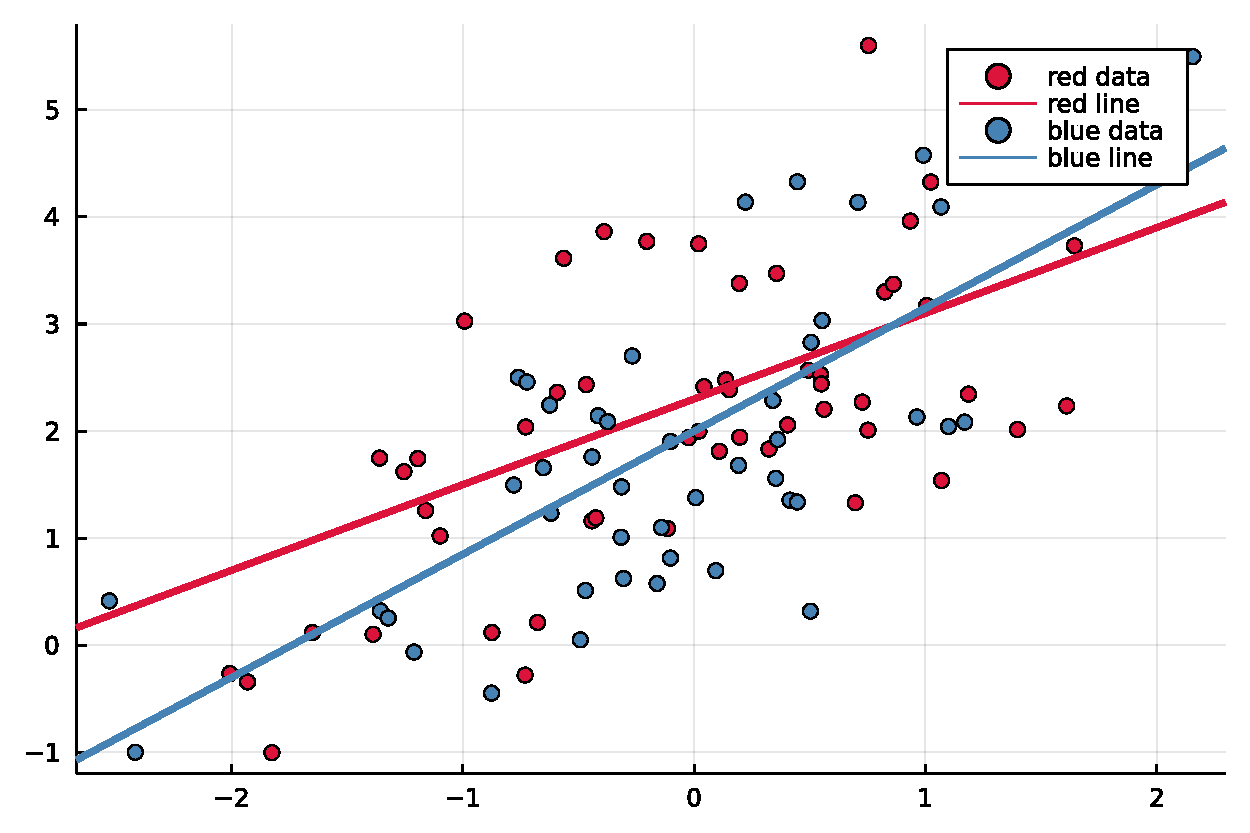
\includegraphics[width=0.8\textwidth]{figures/plot_interaction.pdf}
  \end{figure}
\end{frame}

\begin{frame}[fragile]
  \begin{minted}[autogobble,fontsize=\footnotesize]{julia}
    @model function interaction_model(N, xs, ys, teams)
        a ~ filldist(Normal(0.0, 0.5), 2)

        b ~ filldist(Normal(0.0, 0.5), 2)

        sigma ~ Exponential(1.0)

        for i in 1:N
            if teams[i] == 1.0
                mu_1 = a[1] * xs[i] + b[1]
                ys[i] ~ Normal(mu_1, sigma)
            else
                mu_2 = a[2] * xs[i] + b[2]
                ys[i] ~ Normal(mu_2, sigma)
            end
        end
    end
  \end{minted}
\end{frame}

\section{Analysing Experiments}

\begin{frame}
  How to make my programs faster?

  \pause
  It \textbf{depends}

  \pause
  Depends on what?
\end{frame}

\begin{frame}
  \center
  \begin{tikzpicture}[thick,>=Stealth]
    \node[] (collection) at (-4,1.0) {Collection type};
    \node[] (perf) at (0,1.0) {Execution time};
    \node[] (hardware) at (4,1.0) {Hardware};
    \node[] (usage) at (-4,0) {Collection usage};
    \node[] (compiler) at (4,0) {Compiler};
    \node[] (runtime) at (0,-2) {Runtime};

    \draw[->] (collection) -- (perf.west);
    \draw[->] (usage) -- (perf);
    \draw[->] (hardware.west) -- (perf.east);
    \draw[->] (runtime) -- (perf);
    \draw[->] (compiler) -- (perf);
  \end{tikzpicture}
\end{frame}

\begin{frame}
  \center
  \begin{tikzpicture}[thick,>=Stealth]
    \node[] (collection) at (-4,1.0) {Collection type};
    \node[] (perf) at (0,1.0) {Execution time};
    \node[] (hardware) at (4,1.0) {Hardware};
    \node[] (usage) at (-4,0) {Collection usage};
    \node[] (compiler) at (4,0) {Compiler};
    \node[] (jit-compilation) at (0, -0.5) {JIT-compilation};
    \node[] (runtime) at (0,-2) {Runtime};

    \draw[->] (collection) -- (perf.west);
    \draw[->] (usage) -- (perf);
    \draw[->] (hardware.west) -- (perf.east);
    \draw[->] (runtime) -- (jit-compilation);
    \draw[->] (jit-compilation) -- (perf);
    \draw[->] (compiler) -- (perf);
  \end{tikzpicture}
\end{frame}

\begin{frame}
  \center
  \begin{tikzpicture}[thick,>=Stealth]
    \node[] (collection) at (-4,1.0) {Collection type};
    \node[] (perf) at (0,1.0) {Execution time};
    \node[] (hardware) at (4,1.0) {Hardware};
    \node[] (usage) at (-4,0) {Collection usage};
    \node[] (compiler) at (4,0) {Compiler};
    \node[] (jit-compilation) at (0, -0.5) {Warmup};
    \node[] (runtime) at (0,-2) {JVM};

    \draw[->] (collection) -- (perf.west);
    \draw[->] (usage) -- (perf);
    \draw[->] (hardware.west) -- (perf.east);
    \draw[->] (runtime) -- (jit-compilation);
    \draw[->] (jit-compilation) -- (perf);
    \draw[->] (compiler) -- (perf);
  \end{tikzpicture}
\end{frame}

\begin{frame}
  \center
  \begin{tikzpicture}[thick,>=Stealth]
    \node[] (collection) at (-4,0.0) {Collection type};
    \node[] (perf) at (0,0.0) {Execution time};
    \node[] (hardware) at (4,0.0) {Hardware};
    \node[] (warmup) at (0, -2) {JVM Warmup};

    \draw[->] (collection) -- (perf.west);
    \draw[->] (hardware.west) -- (perf.east);
    \draw[->] (warmup) -- (perf);
  \end{tikzpicture}

  \pause
  \begin{itemize}
  \item \textbf{Machines:} Athena, Hades, Hera
  \item \textbf{Warmup:} Startup (cold JVM), Steady-state (warm JVM)
  \item \textbf{Treatments:} 0->arraylist, 1->arraymap, ...
    \begin{itemize}
    \item Allocation site: 0, 1, 2, ...
    \item Collection: hashmap, arraylist, ...
    \end{itemize}
  \end{itemize}
\end{frame}

\begin{frame}
  \begin{figure}[ht]
    \centering
    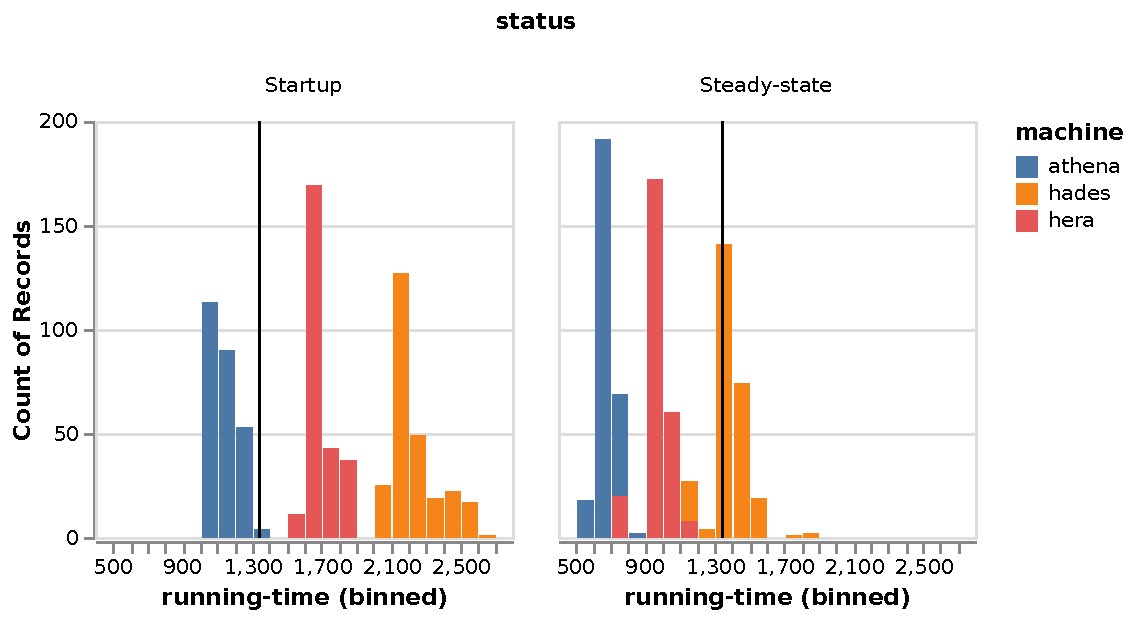
\includegraphics[width=0.9\textwidth]{figures/plot_experiment_distributons.pdf}
  \end{figure}
\end{frame}

\begin{frame}[fragile]
  \begin{align*}
    \observed{ET_j} &\sim \text{Normal}(\mu_j, \parameter{\sigma})\\
    \mu_j &= \observed{\overline{ET}} \times \parameter{\alpha}[\observed{M_j}] \times \parameter{\beta}[\observed{W_j}] \times \markmath{arrayaccess}{\parameter{\gamma}[\observed{T_j}]}\\
    \markmath{alpha}{\parameter{\alpha_m}} &\sim \normal{0.0, 0.5}\\
    \markmath{beta}{\parameter{\beta_w}} &\sim \normal{0.0, 0.2}\\
    \markmath{gamma}{\parameter{\gamma_t}} &\sim \normal{0.0, 0.2}\\
    \parameter{\sigma} &\sim \exponential{30.0}\\
  \end{align*}

  \begin{tikzpicture}[overlay, thick, >=Stealth]
    \node<2->[right=2cm of arrayaccess] (arrayaccesslabel) {Array access};
    \draw<2->[->] (arrayaccesslabel) -- (arrayaccess);

    \node<3->[left=2cm of alpha] (alphalabel) {Arrays};
    \draw<3->[->] (alphalabel) -- (alpha);
    \draw<3->[->] (alphalabel) -- (beta);
  \end{tikzpicture}

  \begin{itemize}
  \item \parameter{x} Parameter
  \item \observed{x} Observed
  \end{itemize}
\end{frame}

\begin{frame}
  \begin{equation*}
    \log(ab) = \log(a) + \log(b)
  \end{equation*}
\end{frame}

\begin{frame}[fragile]
  \begin{align*}
    \log(\observed{ET_j}) &\sim \text{Normal}(\mu_j, \parameter{\sigma})\\
    \mu_j &= \log(\observed{\overline{ET}}) + \parameter{\alpha}[\observed{M_j}] + \parameter{\beta}[\observed{W_j}] + \markmath{arrayaccess}{\parameter{\gamma}[\observed{T_j}]}\\
    \markmath{alpha}{\parameter{\alpha_m}} &\sim \normal{0.0, 0.5}\\
    \markmath{beta}{\parameter{\beta_w}} &\sim \normal{0.0, 0.2}\\
    \markmath{gamma}{\parameter{\gamma_t}} &\sim \normal{0.0, 0.2}\\
    \parameter{\sigma} &\sim \exponential{1.0}\\
  \end{align*}

  \begin{itemize}
  \item \parameter{x} Parameter
  \item \observed{x} Observed
  \end{itemize}
\end{frame}

\begin{frame}
  \begin{figure}[ht]
    \centering
    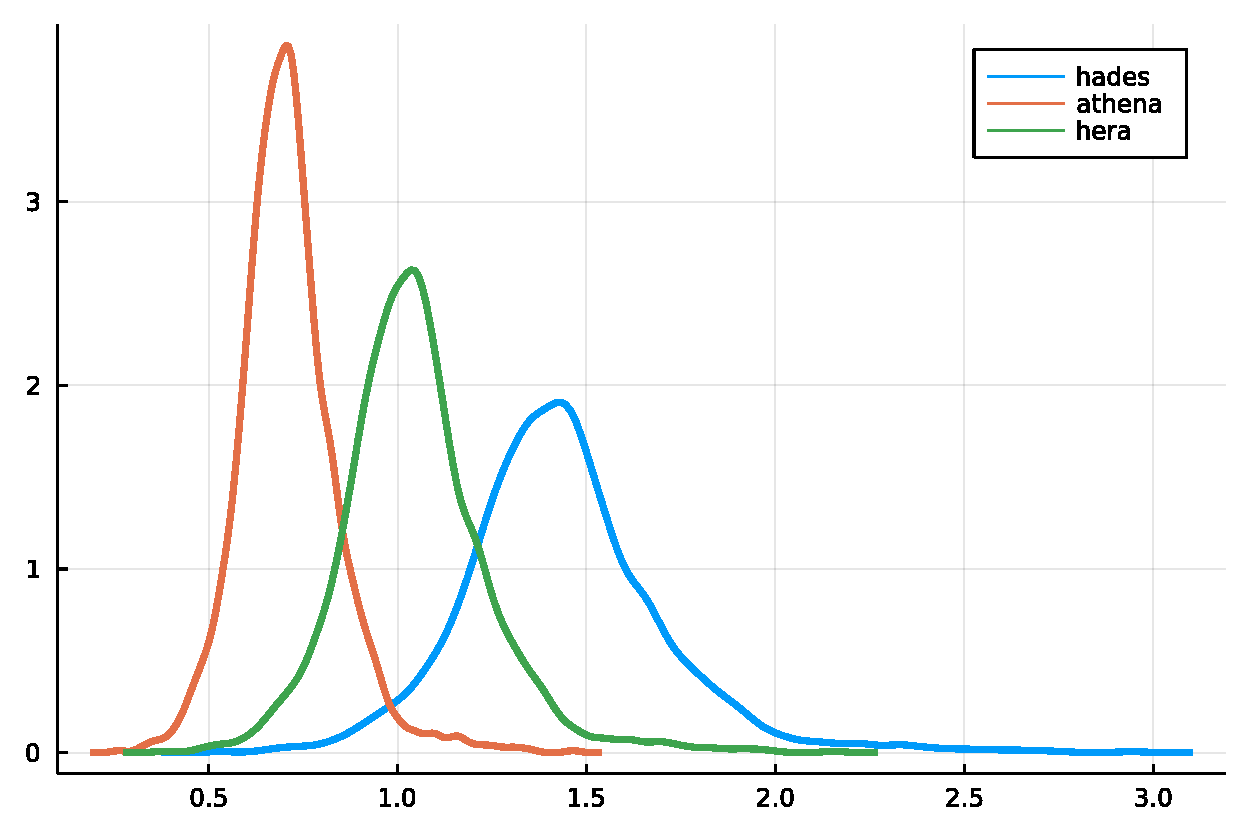
\includegraphics[width=0.7\textwidth]{figures/plot_family_distribution_bloat.pdf}
    \caption{Effect of machine}
  \end{figure}
\end{frame}

\begin{frame}
  \begin{figure}[ht]
    \centering
    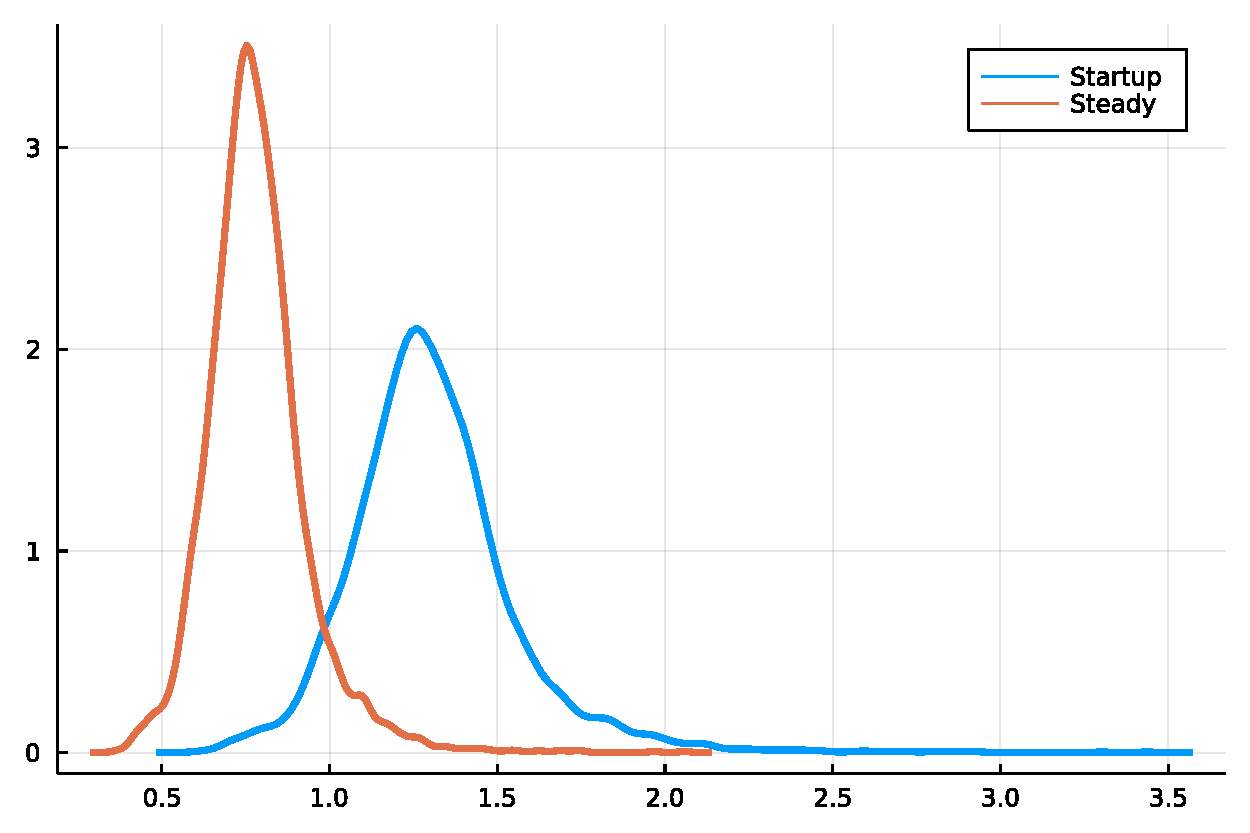
\includegraphics[width=0.7\textwidth]{figures/plot_warmup_distribution_bloat.pdf}
    \caption{Effect of warmup}
  \end{figure}
\end{frame}

\begin{frame}
  \begin{figure}[ht]
    \centering
    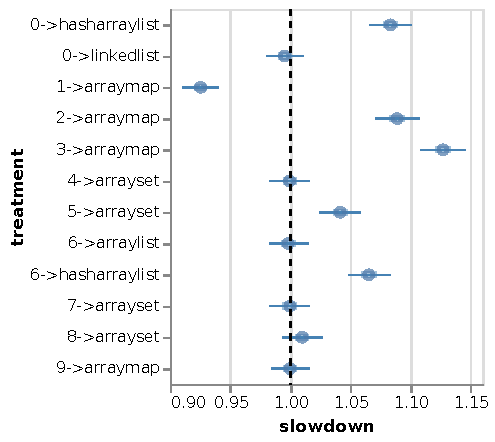
\includegraphics[width=0.5\textwidth]{figures/plot_effects_no_interaction_bloat.pdf}
    \caption{Effect of treatment}
  \end{figure}
\end{frame}

\begin{frame}
  \begin{block}{(Discrete) Interactions}
    Transform an \textbf{array} of coefficients into a \textbf{matrix}
  \end{block}
\end{frame}

\begin{frame}
  \begin{align*}
    \log(\observed{ET_j}) &\sim \text{Normal}(\mu_j, \parameter{\sigma})\\
    \mu_j &= \log(\observed{\overline{ET}}) + \parameter{\alpha}[\observed{M_j}] + \parameter{\beta}[\observed{W_j}] + \parameter{\gamma^{M}}[\observed{M_j}, \observed{T_j}] + \parameter{\gamma^{W}}[\observed{W_j}, \observed{T_j}]\\
    \markmath{alpha}{\parameter{\alpha_m}} &\sim \normal{0.0, 0.5}\\
    \markmath{beta}{\parameter{\beta_w}} &\sim \normal{0.0, 0.2}\\
    \markmath{gamma}{\parameter{\gamma^{W}_{w,t}}} &\sim \normal{0.0, 0.2}\\
    \markmath{gamma}{\parameter{\gamma^{M}_{m,t}}} &\sim \normal{0.0, 0.2}\\
    \parameter{\sigma} &\sim \exponential{1.0}\\
  \end{align*}

  \begin{itemize}
  \item \parameter{x} Parameter
  \item \observed{x} Observed
  \end{itemize}
\end{frame}

%\begin{frame}
%  \begin{columns}
%    \begin{column}{0.5\textwidth}
%      \begin{align*}
%        \log(\observed{ET_j}) &\sim \text{Normal}(\mu_j, \parameter{\sigma})\\
%        \mu_j &= \parameter{\alpha}[\observed{M_j}] + \markmath{arrayaccess}{\parameter{\beta}[\observed{C_j}]}\\
%        \markmath{alpha}{\parameter{\alpha_i}} &\sim \normal{0.0, 0.5}\\
%        \markmath{beta}{\parameter{\beta_i}} &\sim \normal{0.0, 0.2}\\
%        \parameter{\sigma} &\sim \exponential{1.0}\\
%      \end{align*}
%
%      \begin{tikzpicture}[minimum size=1cm]
%        \node[draw] at (-1, 0) {$\alpha_1$};
%        \node[draw] at (0, 0) {$\alpha_2$};
%
%        \node[draw] at (-1, -1) {$\beta_1$};
%        \node[draw] at (0, -1) {$\beta_2$};
%        \node[draw] at (1, -1) {$\beta_3$};
%      \end{tikzpicture}
%    \end{column}
%
%    \begin{column}{0.5\textwidth}
%      \begin{align*}
%        \log(\observed{ET_j}) &\sim \text{Normal}(\mu_j, \parameter{\sigma})\\
%        \mu_j &= \parameter{\gamma}[\observed{M_j}, \observed{C_j}]\\
%        \parameter{\gamma_{m,c}} &\sim \normal{0.0, 0.5}\\
%        \parameter{\sigma} &\sim \exponential{1.0}\\
%      \end{align*}
%
%      \begin{tikzpicture}[minimum size=1cm]
%        \node[draw] at (-1, 0) {$\gamma_{1,1}$};
%        \node[draw] at (0, 0) {$\gamma_{1,2}$};
%        \node[draw] at (1, 0) {$\gamma_{1,3}$};
%
%        \node[draw] at (-1, -1) {$\gamma_{2,1}$};
%        \node[draw] at (0, -1) {$\gamma_{2,2}$};
%        \node[draw] at (1, -1) {$\gamma_{2,3}$};
%      \end{tikzpicture}
%    \end{column}
%  \end{columns}
%\end{frame}

\begin{frame}
  \begin{figure}[ht]
    \centering
    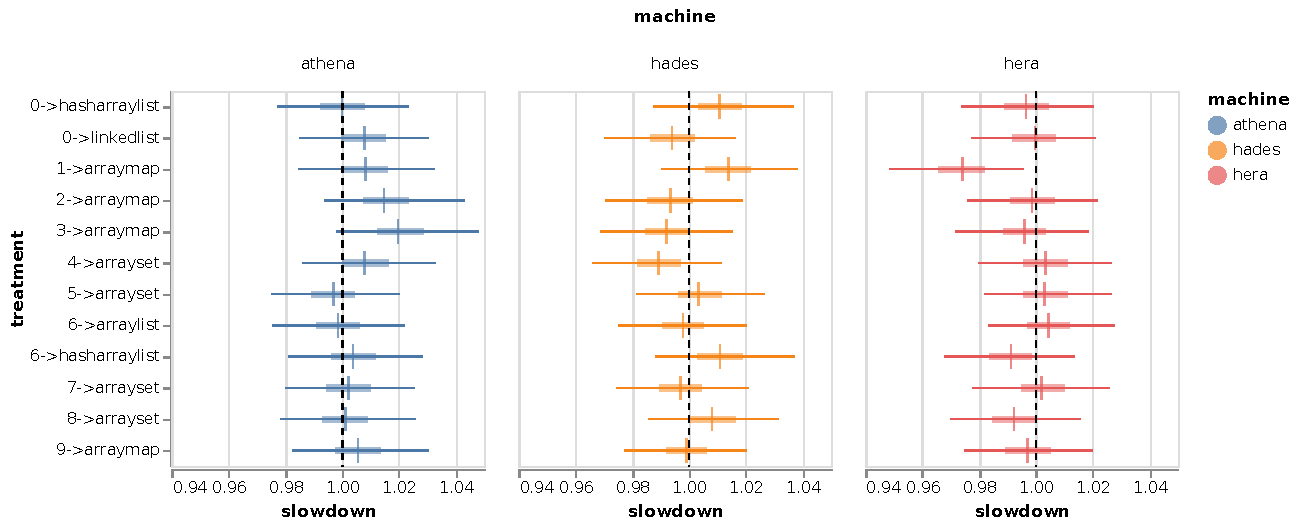
\includegraphics[width=\textwidth]{figures/plot_effect_machine_bloat.pdf}
  \end{figure}
\end{frame}

\begin{frame}
  \begin{figure}[ht]
    \centering
    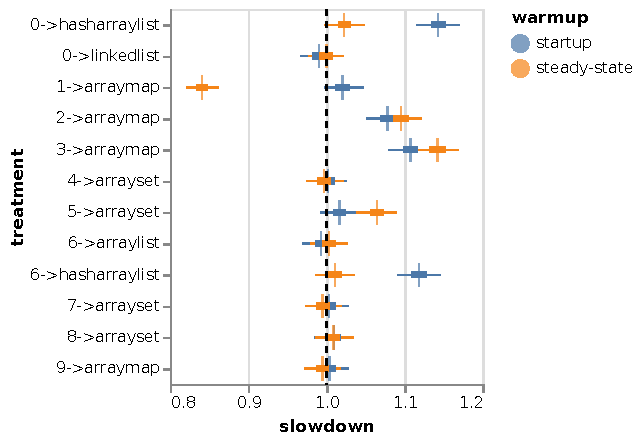
\includegraphics[width=0.7\textwidth]{figures/bayesian-estimate-context-warmup-bloat.pdf}
  \end{figure}
\end{frame}

\section{Hierarchical Models}

\begin{frame}
  \center
  \textbf{Hyperpriors}

  {Priors can have parameters too}

  \pause

  \huge
  {\emoji{exploding-head}}

  % \emph{Hyperpriors} are priors which are \emph{partially} learned from the data.
\end{frame}

\begin{frame}
  \begin{figure}[ht]
    \centering
    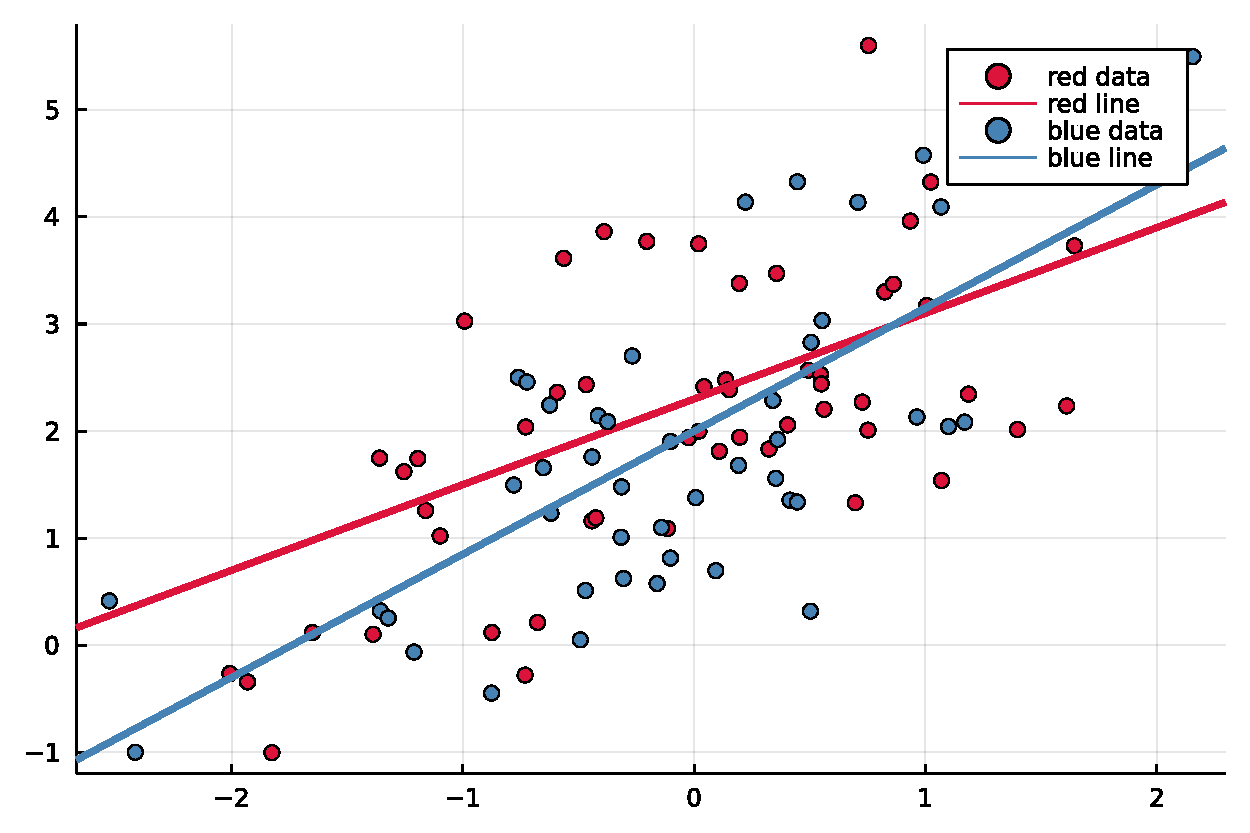
\includegraphics[width=0.8\textwidth]{figures/plot_interaction.pdf}
  \end{figure}
\end{frame}

\begin{frame}[fragile]
  \begin{minted}[autogobble,fontsize=\footnotesize]{julia}
    @model function interaction_model(N, xs, ys, teams)
        a ~ filldist(Normal(0.0, 0.5), 2)

        b ~ filldist(Normal(0.0, 0.5), 2)

        sigma ~ Exponential(1.0)

        for i in 1:N
            if teams[i] == 1.0
                mu_1 = a[1] * xs[i] + b[1]
                ys[i] ~ Normal(mu_1, sigma)
            else
                mu_2 = a[2] * xs[i] + b[2]
                ys[i] ~ Normal(mu_2, sigma)
            end
        end
    end
  \end{minted}
\end{frame}

\begin{frame}[fragile]
  \begin{minted}[autogobble,fontsize=\footnotesize]{julia}
    @model function interaction_model(N, xs, ys, teams)
        sigma_slopes ~ Exponential(0.1)
        a ~ filldist(Normal(0.0, sigma_slopes), 2)

        b ~ filldist(Normal(0.0, 0.5), 2)

        sigma ~ Exponential(1.0)

        for i in 1:N
            if teams[i] == 1.0
                mu_1 = a[1] * xs[i] + b[1]
                ys[i] ~ Normal(mu_1, sigma)
            else
                mu_2 = a[2] * xs[i] + b[2]
                ys[i] ~ Normal(mu_2, sigma)
            end
        end
    end
  \end{minted}
\end{frame}

\begin{frame}
  \begin{block}{Why hyperpriors}
    \begin{itemize}
    \item Prevent overfitting
    \item Use \emph{all} the data
    \end{itemize}
  \end{block}
\end{frame}

\section{Conclusion}

\begin{frame}
  \begin{block}{Bayesian inference is:}
  \begin{itemize}
  \item \textbf{intuitive:} Use probability distributions, no need to learn specific vocabulary
  \item \textbf{flexible:}
    \begin{itemize}
    \item Use the distributions you want
    \item Use the code you want
    \end{itemize}
  \item \textbf{honest:} If not enough data, you get the priors back
  \item \textbf{explicit:} All your assumptions are visible
  \item<2-> Sometimes \textbf{slow}
  \end{itemize}
  \end{block}
\end{frame}

\begin{frame}
  \begin{block}{My Stats Workflow}
    \begin{enumerate}
    \item Generate some fake data (makes you think about what causes what)
    \item Make a statistical model
    \item Test if the model can recover parameters
    \item Use it on experimental data
    \end{enumerate}
  \end{block}
\end{frame}

\begin{frame}
  \begin{block}{Toys to Play With}
    \begin{itemize}
    \item Stan (Standalone DSL)
    \item Turing (Julia)
    \item Pyro (Python, supported by Uber)
    \item Bean Machine (Python, supported by Meta)
    \item Tensorflow Probability (Python, supported by Google)
    \item PyMC3 (Python)
    \end{itemize}
  \end{block}
\end{frame}

\begin{frame}
  \begin{block}{Books to Read}
  \begin{itemize}
  \item Bayesian Methods for Hackers
  \item Statistical Rethinking (McElreath)
  \item Causal Inference In Statistics, a primer (Pearl, Glymour, Jewell)
  \end{itemize}
  \end{block}
\end{frame}

\begin{frame}
  \centering
  Thanks!
\end{frame}

\section{Extra Slides}

\section{Prior Sensitivity Analysis}

\begin{frame}{The Idea}
  \center
  Try out different priors, and check how predictions change!
\end{frame}

\section{Causal Inference}

\begin{frame}
  \center
  \huge
  Correlation isn't causation

  \footnotesize
  (But then what is causation?)
\end{frame}

\begin{frame}
  \center
  \huge
  Causation

  \small
  X causes Y if Y relies on X for its value
\end{frame}

\begin{frame}
  How can correlation appear?
  \begin{itemize}
  \item X causes Y
  \item Y causes X
  \item X and Y share common cause Z (Confounding)
  \item Selection bias (Colliders)
  \end{itemize}
\end{frame}

\begin{frame}
  \center
  \huge
  Direct causes

  \begin{tikzpicture}[thick, >=Stealth]
    \node (x) at (-1, 0) {X};
    \node (y) at (1, 0) {Y};

    \draw[->] (x) -- (y);
  \end{tikzpicture}

  \begin{tikzpicture}[thick, >=Stealth]
    \node (x) at (-1, 0) {X};
    \node (y) at (1, 0) {Y};

    \draw[->] (y) -- (x);
  \end{tikzpicture}
\end{frame}

\begin{frame}{Confounding}
  \center
  \begin{tikzpicture}[thick,>=Stealth]
    \node (tobacco) at (-2, 0) {Tobacco};
    \node (cancer) at (2,0) {Cancer};

    \draw[->] (tobacco) -- (cancer) node[midway, above] {?};
  \end{tikzpicture}
\end{frame}

\begin{frame}{Confounding}
  \center
  \begin{tikzpicture}[thick,>=Stealth]
    \node (tobacco) at (-2, 0) {Tobacco};
    \node (cancer) at (2,0) {Cancer};
    \node (genes) at (0, 2) {Genetic Factors};

    \draw[->] (tobacco) -- (cancer) node[midway, above] {?};
    \draw[->] (genes) -- (tobacco);
    \draw[->] (genes) -- (cancer);
  \end{tikzpicture}
\end{frame}

\begin{frame}
  \begin{center}
    Confounder (or Fork)

    \begin{tikzpicture}[thick, >=Stealth]
        \node (x) at (-1, 0) {X};
        \node (y) at (1, 0) {Y};
        \node (z) at (0, 1) {Z};

        \draw[->] (z) -- (x);
        \draw[->] (z) -- (y);
    \end{tikzpicture}

  \end{center}
\end{frame}

\begin{frame}
\begin{center}
  \huge
  Collider

  \begin{tikzpicture}[thick, >=Stealth]
    \node (x) at (-1, 0) {X};
    \node (y) at (1, 0) {Y};
    \node (z) at (0, -1) {Z};

    \draw[->] (x) -- (z);
    \draw[->] (y) -- (z);
  \end{tikzpicture}
\end{center}
\end{frame}



\end{document}
